\documentclass[a4paper,11pt,xcolor=dvipsnames]{scrreprt}

\usepackage[ngerman]{babel}
\usepackage[utf8]{inputenc}
\usepackage[T1]{fontenc}
\usepackage{graphicx}
\usepackage{amsmath,amssymb,amsthm}
\usepackage[tracking=true]{microtype}
\usepackage{lmodern}
\usepackage[usenames,dvipsnames]{xcolor}
\usepackage{hyperref}

% ToDo Notes einbinden
% Package für ToDoNotes laden
\usepackage
[german
,colorinlistoftodos
,textwidth=60
%,disable %nur wenn finale Abgabe einkommentieren
]
{todonotes}

% Usage:	\todo[color=<farbe>]{ToDoNote-Text}
% Farben:	- Red:		noch offener Punkt
%			- RubineRed:noch offenes Feature (nicht ganz so große Prio)
%			- Orange:	in Bearbeitung
%			- Green:	fertig bearbeitet
%			- Blue:		Veränderter Inhalt reviewed
% Wenn der Inhalt und die Grammatik überprüft wurde kann die ToDoNote gelöscht
% werden


% Boxen einfügen
% Farben definieren (Nicht gebrauchtes auskommentieren):
% Online-Version
%\colorlet{BoxBackground}{LimeGreen!100!}
\definecolor{BoxBackground}{HTML}{83EF03}	% Boxen in Lambda-Pi Farbe (siehe
% Logo)
\colorlet{BoxBorderframe}{Black!100!}

% Druckversion
%\colorlet{BoxBackground}{Gray!70!}
%\colorlet{BoxBorderframe}{Black!100!}


% Boxen definieren
%
% Usage: \<command{%
% 	<input>
%}
%
% Formel Boxen
\newcommand{\formel}[1]{
	\\
	\fcolorbox{BoxBorderframe}{BoxBackground}{%
		\parbox{%0.87
		\linewidth}{%
			#1
		}
	}
	\\
}

% Zusammenfassung
\newcommand{\summary}[1]{
	\begin{center}
	\fcolorbox{BoxBorderframe}{BoxBackground}{%
		\parbox{\linewidth}{%
			\large{\textbf{Zusammenfassung:}}\\
			#1
		}
	}
	\end{center}
}

% Signalwörter
\newcommand{\tags}[1]{
	\begin{center}
	\fcolorbox{BoxBorderframe}{BoxBackground}{%
		\parbox{\linewidth}{%
			\large{\textbf{Signalwörter:}}\\
			#1
		}
	}
	\end{center}
}

\title{Skript zum Mathe - Abi-Vorbereitungskurs~2015\\
	
\includegraphics[scale=0.15]{Images/Logo.jpg}
	\author{Jan, Lucas \& Patrick\\
	www.lambda-pi.de}
	\date{\today}}

\usepackage{amsmath}

\begin{document}

	% Titelseite einfügen
	\maketitle
	\newpage

	% Liste der ToDo's erzeugen
	\listoftodos
	
	% Inhaltsverzeichnis einf�gen
	\tableofcontents
	\newpage
	
	\todo[color=green]{In allen Teilen ToDo's für die Umstrukturierung einfügen}
	\todo[color=green]{Einzelne Sektionen mit kurzer Zusammenfassung}
	\todo[color=green]{Einzelne Sektionen mit Signalwörter}
	% Vorwort 
	\chapter*{Vorwort}
	\todo[inline,color=red]{Vorwort nach Umstrukturierung des Skripts erneuern (pt)}
	Dieses Skript soll unterstützend zu unserem Abi-Vorbereitungskurs in Mathematik
	in Baden-Württemberg gelten. Wir haben versucht den Stoff für das Abitur auf
	das Wesentliche zu konzentrieren und hier als Nachschlagewerk zusammenzufassen.
	Wir erheben keinen Anspruch auf Vollständigkeit, aber es sollte alles vorhanden
	sein was ihr für das Mathe-Abi braucht. Sollte dem nicht so sein oder euch
	Fehler auffallen, dann gebt uns bitte Bescheid, damit wir diese beheben können
	;).\\
	Wir möchten noch erwähnen, dass wir hier an einigen Stellen bewusst Sachen
	nicht 100\%ig mathematisch korrekt benannt haben. Das hat aber den Hintergrund,
	dass uns die Didaktik und das Verständnis des Stoffes wichtiger sind, als die
	mathematisch korrekten Definitionen. Wir haben aber versucht, alles - für das
	Abitur ausreichend korrekt - zu beschreiben. Ansonsten hoffen wir, dass euch
	der Kurs ein paar Notenpunkte extra bringt und ihr auch sonst ein erfolgreiches
	Abitur schreibt :).\\
	Das Skript steht unter der '\textbf{GNU Free Documentation License}, Version
	1.3', das heißt, das Skript steht allen frei zur Verfügung und darf unter
	Nennung der Autoren (bzw. unserer Internetseite \url{http://www.lambda-pi.de})
	verbreitet und verändert werden, sofern diese Lizenz beibehalten wird. Das
	heißt ihr dürft das Skript nicht nur kostenlos weitergeben sondern auch
	verbessern und so verändern wie ihr wollt. Die Lizenz ist unter anderem hier
	veröffentlicht:\\
	\url{http://www.gnu.org/licenses/fdl-1.3.html}
	
	\todo[inline,color=red]{Kapitel "Aufbau des Skripts" einfügen}
	\todo[inline,color=red]{Kapitel "Strukturiertes lösen von Aufgaben" einfügen}
	
	% Wiederholungen und Vorgeplänkel
	\chapter{Wiederholungen \& Vorgeplänkel}
Hier möchten wir auf die grundlegenden, mathematischen Vorkenntnisse aus der Mittelstufe zurückgreifen und einige Dinge aus der Oberstufe vorziehen, um eine solide Grundlage für die eigentlichen späteren Themen zu legen.
% Chapters/Wiederholungen/
% Mengenlehre
\section{Mengenlehre}
 	\todo[color=purple]{Kasten für Formel hinzufügen}
 	\todo[color=purple]{Zusammenfassung-Kasten hinzufügen}
 	\todo[color=purple]{Signalwörter-Kasten hinzufügen}
	Dieser Teil wird zwar im Abitur nicht explizit abgefragt, aber kann einige
	Probleme, die viele unserer Nachhilfeschüler hatten, auflösen.\\
	Gerade um Aufgaben in der Wahrscheinlichkeitsrechnung besser verstehen zu
	können, ist es von Vorteil, ein Verständnis von Mengen zu haben.

	\subsection{Definition}
 		\todo[color=purple]{Kasten für Formel hinzufügen}
 		\todo[color=purple]{Zusammenfassung-Kasten hinzufügen}
 		\todo[color=purple]{Signalwörter-Kasten hinzufügen}
		Mengen sind keine Zahlen oder Symbole, aber eine Menge kann diese als Elemente
		beinhalten. Letztendlich werden Mengen benutzt, um bestimmte Dinge
		(Elemente, Zahlen, die unterschiedlichen Schüler,\ldots) zu gruppieren und
		zusammenzufassen. Ihr kennt das bereits aus der 7. Klasse. Dort musste man
		beim Lösen von Gleichungen immer die Lösungsmenge \(L\) angeben. Diese sah
		dann möglicherweise wie folgt aus: \(L:=\{2,\ 3,\ 5\}\). \(2,\ 3,\ 5\) heißen
		dann auch Elemente der Lösungsmenge \(L\).\\
		Noch anzumerken ist, dass auch \(\textit{rot}\), \(\textit{schwarz}\),
		\(\textit{Kopf}\), \(\textit{Zahl}\),\(\cdots\) Elemente einer Menge sein
		können.\\

	\subsection{Wichtige Eigenschaften von Mengen}
 		\todo[color=purple]{Kasten für Formel hinzufügen}
 		\todo[color=purple]{Zusammenfassung-Kasten hinzufügen}
 		\todo[color=purple]{Signalwörter-Kasten hinzufügen}
			Auch für Mengen gibt es Rechenregeln. Die wichtigsten, zumindest die, die wir
			brauchen, sind hier kurz zusammengefasst.
			\subsubsection{Komplement - in der Statistik oft Gegenmenge}
				Das Komplement einer Menge sind alle Elemente, die nicht in dieser Menge
				enthalten sind. Hat man zum Beispiel die geraden Zahlen des Würfels
				\(A=\{2,\ 4,\ 6\}\), so ist das Komplement die Menge, mit allen ungeraden
				Zahlen \(\bar{A}=\{1,\ 3,\ 5\}\).
			\subsubsection{Mächtigkeit}
				Später ist es interessant zu wissen, wie viele Elemente eine Menge enthält.
				Dafür müssen wir 'den Betrag' der Menge betrachten. Anders als bei Zahlen
				heißt dieser hier Mächtigkeit.\\
				Die Mächtigkeit der Menge der geraden Zahlen eines Würfels wäre dann
				\(|A|=3\), da die Menge aus drei Elementen besteht.


% Ausblick in die Zahlentheorie
\section{kurzer Ausblick in die Zahlentheorie}
	\todo[color=purple]{Kasten für Formel hinzufügen}
	\todo[inline,color=red]{Zusammenfassung-Kasten hinzufügen}
	\todo[inline,color=red]{Signalwörter-Kasten hinzufügen}
	Zuerst möchten wir noch einmal auf die unterschiedlichen Zahlenmengen eingehen:\\
	
	\(\star\) Die natürlichen Zahlen: \(\mathbb{N}=\{1,2,3,\cdots\}\) \\
	
	\(\star\) Oft wird auch \(\mathbb{N}_0\) als Zahlenbereich angegeben:
	\(\mathbb{N}_0=\mathbb{N}\cup\{0\}\)\\
	
	\(\star\) Bei den ganzen Zahlen kommen noch negative Zahlen dazu:
	\(\mathbb{Z}=\{0,\mp 1,\mp 2,\mp 3,\cdots\}\) \\
	
	\(\star\) Die rationalen Zahlen lassen sich als Bruch einer natürlichen Zahl
	und einer ganzen Zahl darstellen, mit \(a\in\mathbb{N}\) und \(b\in\mathbb{Z}\)
	gilt: \(\frac{a}{b}\):
	\(\mathbb{Q}=\{-2,-\frac{1}{3},0,\frac{1}{2},1,\cdots\}\) \\
	
	$\star$ Man könnte meinen damit ist jeder Platz auf dem Zahlenstrahl belegt,
	aber es finden sich immer noch Plätze für Zahlen wie \(\pi\), \(\sqrt{2}\) und
	\(e\).
	Diese Zahlen heißen irrational, weil sie nicht zu den rationalen Zahlen
	\(\mathbb{Q}\) gehören. Mit den irrationalen Zahlen allein wird so gut wie nie
	gerechnet. Dargestellt werden die irrationalen Zahlen deshalb auch selten
	allein, man nimmt dafür \(\mathbb{I}\).\\

	\(\star\) Zuletzt noch die reellen Zahlen, welche alle Zahlenmengen davor
	beinhaltet. Also rein formell
	\(\mathbb{R}=\mathbb{N}\cup\mathbb{N}_0\cup\mathbb{Z}\cup\mathbb{Q}\cup\mathbb{I}\).
	Da aber \(\mathbb{Q}=\mathbb{N}\cup\mathbb{N}_0\cup\mathbb{Z}\) usw. gilt,
	schreibt man \(\mathbb{R}=\mathbb{Q}\cup\mathbb{I}\). \\ \\
	
	Grundsätzlich dürfen wir jede dieser Zahlenmengen nutzen. Meistens nutzen wir
	jedoch \(\mathbb{R}\), welche alle Zahlen einschließt, die ihr kennt. \\
	Wie können wir die Zahlen nun einsetzen? Dazu gibt es grundsätzlich zwei
	Möglichkeiten. Als Variablen oder Faktoren(/Konstanten\footnote{Der Unterschied
	ist hier nicht so wichtig, wir werden daher diese Begriffe als gleichwertig
	betrachten.}).\\
	
	\(\star\) Variablen kennen wir von Funktionen wie f(x). Bei f(x) stellt x die
	Variable der Funktion dar. Diese läuft alle Zahlen durch und nimmt jede
	mögliche Zahl an. Daraus ergibt sich dann jeweils ein Funktionswert f(x). Haben
	wir alle Funktionswerte zu jedem Wert der Variablen, so haben wir die Funktion
	komplett gezeichnet (sofern man die Werte einzeichnet). \\
	
	\(\star\) Was hat es nun mit den Faktoren auf sich? Diese stehen als Zahl
	alleine oder mit einer Variablen zusammen. Sie bilden einfach eine Zahl ab, die
	multipliziert, addiert oder sonst was wird. Entscheidend ist, dass dies auch so
	bleibt, wenn wir die Zahl nicht kennen und ihr deshalb einen Namen, wie zum
	Beispiel ein a oder c, geben.\\
	Variablen sind also Elemente, welche alle möglichen Werte annehmen können.
	Faktoren dagegen stehen als eine eindeutige Zahl da, unabhängig davon, wie sie
	dargestellt ist.
	Gleichzeitig dürfen wir Zahlen, auch ohne Buchstaben zu nutzen, verschieden
	darstellen. Ob wir \(2+2+2\text{ oder }3\cdot 2\) schreiben \textit{oder} 6
	\textit{oder} a (wenn wir die Zahl so nennen wollen) spielt also keine Rolle.
	Alle Ausdrücke sind unterschiedliche Darstellungen für die gleiche Zahl. Diese
	Tatsache kann helfen, Terme anders zu schreiben und sie damit zu
	vereinfachen.\\


% Grundlegende Regeln der Algebra
\section{Grundlegende Regeln der Algebra}
	Zwar sind die kommenden Regeln den meisten (wenn auch nicht nach dem Namen)
	bekannt, der Vollständigkeit halber werden wir sie aber trotzdem kurz erwähnen.
	
	\subsection{Distributivgesetz}
 		\todo[color=purple]{Zusammenfassung-Kasten hinzufügen}
 		\todo[color=purple]{Signalwörter-Kasten hinzufügen}
		\( \) % Bugfix, nur dann geht \formel{}
		\formel{\[a \cdot (b+c) = a \cdot b + a \cdot c\]}
		\\ \\
		Diese Regel gilt auch bei Brüchen!
		\[\frac{a+b}{c}=\frac{1}{c}\cdot (a+b)=\frac{a}{c}+\frac{b}{c}\]
	
	\subsection{Kommutativgesetz}
 		\todo[color=purple]{Zusammenfassung-Kasten hinzufügen}
 		\todo[color=purple]{Signalwörter-Kasten hinzufügen}
		Vertauschung von links \& rechts:
		\\ \\
		\formel{\[a+b=b+a,\ bzw\ a\cdot b=b\cdot a\]}
	
	\subsection{Assoziativgesetz}
 		\todo[color=purple]{Zusammenfassung-Kasten hinzufügen}
		\todo[color=purple]{Signalwörter-Kasten hinzufügen}
		Vernachlässigung der Reihenfolge:
		\\ \\
		\formel{\[(a+b)+c=a+(b+c),\ bzw\ (a\cdot b)\cdot c=a\cdot (b\cdot c)\]}

% Binomische Formeln
\section{Binomische Formeln}
	\todo[color=purple]{Zusammenfassung-Kasten hinzufügen}
	\todo[color=purple]{Signalwörter-Kasten hinzufügen}
	Ab und zu können diese vor allem im Pflichtteil vorkommen, wenn ihr zum
	Beispiel eine Gleichung lösen oder eine Formel vereinfachen sollt. 
	Daher wiederholen wir sie noch einmal:
	\\ \\
	\formel{
		\[\mathrm{1.\ binomische\ Formel:\ }(a+b)^2=a^2+2ab+b^2\]
		\[\mathrm{2.\ binomische\ Formel:\ }(a-b)^2=a^2-2ab+b^2\]
		\[\mathrm{3.\ binomische\ Formel:\ }(a+b)\cdot (a-b)=a^2-b^2\]
	}

% p-q-Formel
\section{p-q-Formel (auch Mitternachtsformel)}
	\todo[color=red]{Kasten für Formel hinzufügen}
	\todo[color=red]{Zusammenfassung-Kasten hinzufügen}
	\todo[color=red]{Signalwörter-Kasten hinzufügen}
	Die p-q-Formel wird immer dann benötigt, wenn wir eine quadratische Gleichung
	der Form \(x^2 + p x + q = 0\) \footnote{Vor dem \(x^2\) darf keine Zahl stehen
	und auf der rechten Seite nur eine 0!} auflösen wollen, wobei p \& q bekannt
	sind. p \& q werden dann einfach in folgende Gleichung
	eingesetzt\footnote{Beachtet bitte immer die Vorzeichen! Wenn z. B. q=-4 ist,
	so steht in der Wurzel ein +!}:
	\[x_{1,2}=-\frac{p}{2}\pm \sqrt{\left ( \frac{p}{2} \right)^2-q}\]


% Potenzregeln
\section{Potenzregeln}
	\todo[color=purple]{Zusammenfassung-Kasten hinzufügen}
	\todo[color=purple]{Signalwörter-Kasten hinzufügen}
	Auch wichtig sind die Potenzregeln. Grundsätzlich gilt:
	\\ \\
	\formel{\[\underbrace{a\cdot a\cdot a\cdot\ldots\cdot a}_{n-Mal}=a^n\]}
	\\ \\ \\ \\ \\ \\
	Des Weiteren ist definiert, dass eine negative Hochzahl den Kehrwert angibt:
	\\ \\
	\formel{\[\frac{1}{x^n}=x^{-n}\]}
	\\ \\
	\(\star\) Kommen wir nun zu den eigentlichen Regeln. Multipliziert man zwei
	Potenzen mit gleicher Basis, so kann man die Exponenten addieren:
	\\ \\
	\formel{\[a^m\cdot a^n=a^{m+n}\]}
	\\ \\
	\(\star\) Schauen wir uns einmal die letzten zwei Regeln an und kombinieren
	sie. \(a^0=a^{n-n}=a^n\cdot a^{-n}=\frac{a^n}{a^n}=1\). Es gilt also:
	\\ \\
	\formel{\[a^0=1,\text{ für }a\neq 0\]}
	\\ \\
	\(\star\) Potenzieren wir eine schon potenzierte
	Zahl, so können wir die Potenzen einfach multiplizieren:
	\\ \\
	\formel{\[\left ( a^n \right )^m=a^{n\cdot m}\]}
	\\ \\
	\(\star\) Aus \(\sqrt{x}^2=\left ( x^{\frac{1}{2}}\right
	)^2=x^{\frac{2}{2}}=x\) können wir uns auch herleiten, wie man eine Wurzel als
	Potenz darstellen kann. Es gilt dann also:
	\\ \\
	\formel{\[\sqrt[n]{x}=x^{\frac{1}{n}}\]}
	\\ \\
	\(\star\) Haben wir die gleichen Exponenten, aber verschiedene Basen, so können
	wir zuerst die Basen multiplizieren und dann weiter rechnen:
	\\ \\
	\formel{\[a^n\cdot b^n=(a\cdot b)^n, \textrm{\ bzw\ } \frac{a^n}{b^n}=\left (
	\frac{a}{b}\right ) ^n\]}


% Bruchrechnen
\section{Bruchrechnen}
	\todo[color=red]{Kasten für Formel hinzufügen}
	\todo[color=red]{Zusammenfassung-Kasten hinzufügen}
	\todo[color=red]{Signalwörter-Kasten hinzufügen}
	Wir haben oftmals die Erfahrung gemacht, dass einige Schüler Probleme mit dem
	Bruchrechnen haben. Kommt man damit jedoch klar, so kann man sich viel Zeit im
	Pflichtteil ersparen und einige Rechnungen stark vereinfachen. \\
	
	\(\star\) Wie wir schon beim Distributivgesetz angesprochen hatten, gilt
	\[\frac{a+b}{c}=\frac{a}{c}+\frac{b}{c}\]
	
	\(\star\) Auch ein wichtiger Punkt, den wir ansprechen wollen, betrifft das
	Teilen durch einen Bruch. Haben wir zum Beispiel die Gleichung
	
	\(\frac{2}{4}\cdot x=4\) und wollen nach x auflösen, so müssen wir durch den
	Bruch teilen. \emph{Das ist aber das Gleiche wie das Produkt mit dem Kehrwert
	zu wählen!} Es gilt dann nämlich \(\frac{4}{2}\cdot \frac{2}{4}\cdot
	x=\frac{4}{2}\cdot 4\) und der Bruch kürzt sich einfach weg, auf der linken
	Seite.\\
	
	\(\star\) Noch kurz zum Vorteil der Schreibweise von Brüchen. Es gilt \(2\cdot
	\frac{1}{3}=\frac{2}{3}\). Der Vorteil, wenn man Zahlen als Bruch schreibt,
	anstatt als Dezimalzahl, liegt unter anderem daran, dass man leicht kürzen
	kann. Einzusehen dass \(6\cdot \frac{1}{3}=2\) ist deutlich einfacher als
	\(6\cdot 0,\widetilde{3}=2\).\\
	
	\(\star\) Zu guter Letzt kommen wir noch kurz auf das Addieren von Brüchen zu
	sprechen. Zuerst muss man den kleinsten gemeinsamen Nenner finden (in dem als
	Produkt aller Primzahlen dargestellt, sich beide Nenner finden lassen) und die
	Brüche dann auf diesen erweitern. Die Zähler werden dann einfach wie gewohnt
	addiert, während der Nenner gleich bleibt (siehe auch das Distributivgesetz bei
	Brüchen).


% Gleichungen auflösen
\section{Gleichungen auflösen}
\todo[color=red]{Kasten für Formel hinzufügen}
\todo[color=red]{Zusammenfassung-Kasten hinzufügen}
\todo[color=red]{Signalwörter-Kasten hinzufügen}
Dieses Kapitel ist Fundamental für das komplette Mathe-Abitur. Egal ob wir Funktionen aufstellen, ein lineares Gleichungssystem (kurz LGS) im Geometrieteil lösen oder auch bei einigen anderen Aufgaben im Pflichtteil (ansonsten Übernimmt unser CAS-Taschenrechner diese Aufgaben) muss man Gleichungen auflösen. Die Palette an Anwendungen sollte also Motivation genug sein, sich hier noch einmal ausgiebig damit zu beschäftigen.\\
\(\star\)Das Wichtigste beim Auflösen einer jeden Gleichung ist, dass bei jedem Rechenschritt auf beiden Seiten das Gleiche gemacht werden muss. Grund hierfür ist die Grundüberlegung einer Gleichung. Nehmen wir an, wir haben eine Waage. Steht die Waage im Gleichgewicht, so muss die Masse links genau so groß sein, wie rechts. Wollen wir das Gleichgewicht beibehalten, so müssen wir auch auf beiden Seiten das Gleiche machen. Nehmen wir 5 kg von der einen Seite, so müssen wir das auf der anderen Seite auch tun. Genauso verhält sich das bei Gleichungen. \\
\(\star\)Ein weiterer wichtiger Punkt ist, dass bei allen Gleichungen die wir Teilen / miteinander Mal nehmen / den Logarithmus nehmen / hoch e nehmen / quadrieren / usw., der Rechenschritt mit dem kompletten Term gemacht werden muss. Ein kurzes Beispiel:
\[ln(x+2)=4+b\ |e^{...}\Rightarrow\ x+2=e^{4+b}\]
\(\star\) Um eine (lineare) Gleichung aufzulösen, gehen wir immer von außen nach innen vor\footnote{Leider ist eine komplette Anleitung hier schwer umzusetzen. Wir beschränken uns hier also auf einige wenige Beispiele. Im Kurs selbst werden wir jedoch alle Fälle durchgehen.} Zuerst wird versucht, alle Summanden mit unserer gesuchten Zahl (zum Beispiel x)zuerst auf eine Seite des =, dann auf den Zähler zu bekommen oder aus dem \(e\) oder sonstigen raus zu nehmen (durch die jeweilige Gegenfunktion). Danach haben wir die Gleichung meistens schon so gut wie gelöst. \emph{Haben wir quadratische Gleichungen, so ist natürlich die p-q-Formel zu benutzen.}\\
\(\star\) Schwerer scheint es, wenn e oder trigonometrische Funktionen im Spiel sind, die quadriert werden. Dann substituieren wir einfach, das heißt, wir ersetzen (z. B.) jedes \(e^x\) durch einen Buchstaben (geben ihm also einen Spitznamen ;) ). Zum Beispiel \(e^{2x}+e^x+1=0\ =>\ u^2+u+1=0\text{, für }u=e^x\) \footnote{Vergesst dann bitte nicht u zurück zu substituieren, wenn ihr einen Wert für u habt und dann nach x umzustellen.}


% Gaußverfahren für LGS
\newpage
\section{Gaußverfahren für LGS}
	\todo[color=purple]{Kasten für Formel hinzufügen}
	\todo[color=purple]{Zusammenfassung-Kasten hinzufügen}
	\todo[color=purple]{Signalwörter-Kasten hinzufügen}
	Aus der Mittelstufe wissen wir, wie wir ein LGS mit zwei Variablen auflösen
	können. Wichtig für das Gaußverfahren ist das Additionsverfahren, welches dabei
	benutzt wird. Das Gaußverfahren hat den Vorteil, dass jedes LGS mit beliebig
	vielen Variablen gelöst werden kann. Meistens brauchen wir nur drei Variablen
	oder Gleichungen. Hierzu verwenden wir die Matrix, welche einfach eine andere
	Schreibweise der bekannten Form darstellt. So wird aus 
	\[(I)\ x_1+2x_2+3x_3=2,\
	(II)\ x_1+x_2+x_3=2,\ (III)\ 3x_1+3x_2+x_3=0\]
	\[
	\left(
	 \begin{matrix}
	  1 & 2 & 3\\
	  1 & 1 & 1\\
	  3 & 3 & 1
	 \end{matrix}
	 \left|
	  \begin{matrix}
	   2\\
	   2\\
	   0
	  \end{matrix}
	 \right)
	\right.
	\]
	Die Schreibweise hat aber keinerlei Auswirkungen auf die Lösung. Wir möchten
	nun den Gauß'schen Algorithmus dafür aufschreiben:\\

	\textbf{1. Schritt:} Zunächst schreibt man die erweiterte Matrix auf (erweitert
	wegen dem Strich) oder ihr schreibt die Gleichungen einfach, wie bekannt,
	untereinander. Beachtet bitte, dass alle \(x_1,\ x_2,\ x_3\) jeweils
	untereinander stehen, auf der linken Seite der Gleichung nur Summanden mit x
	stehen und auf der rechten Seite nur die Zahlen! Am besten benennt ihr die
	Zeilen mit römischen Ziffern, um die Rechnung übersichtlich zu halten.\\

	\textbf{2. Schritt:} Wenn möglich, verschiebe die Zeilen so, dass nur in den
	unteren Zeilen eine 0 in der ersten Spalte steht (hier würde dann das \(x_1\)
	in der Gleichung fehlen). Dies ist in unserem Beispiel nicht der Fall, also
	gehen wir über zum\\

	\textbf{3. Schritt:} Ziehe (oder addiere) je nach Zeile das Vielfache von der
	ersten Zeile, zum Vielfachen der anderen Zeilen, so ab, dass an entsprechender
	Stelle eine 0 steht. Die erste Zeile bleibt aber stehen! So würden wir in der
	2. Zeile | (I)-(II) haben, und in der 3. Zeile | 3(I)-(III). Daraus folgt:
	\[
	\left(
	 \begin{matrix}
	  1 & 2 & 3\\
	  0 & 1 & 2\\
	  0 & 3 & 8
	 \end{matrix}
	 \left|
	  \begin{matrix}
	   2\\
	   0\\
	   6
	  \end{matrix}
	 \right)
	\right.
	\]

	\textbf{4. Schritt:} Wiederhole Schritte 2 \& 3 so oft, bis in der letzten
	Zeile lediglich eine Zahl auf der linken Seite übrig bleibt (nur zieht man danach von
	der 2. Zeile ab und lässt diese stehen, usw.). Dann erhalten wir
	(Rechenschritte: 3. Zeile wird berechnet durch 3(II)-(III)):
	\[
	\left(
	 \begin{matrix}
	  1 & 2 & 3\\
	  0 & 1 & 2\\
	  0 & 0 & -2
	 \end{matrix}
	 \left|
	  \begin{matrix}
	   2\\
	   0\\
	   -6
	  \end{matrix}
	 \right)
	\right.
	\]

	\textbf{5. Schritt:} Hat man die Stufenform, gibt es zwei Möglichkeiten. Die
	Erste ist, wir rechnen die unterste Variable einfach aus und setzen sie in die 2.
	Zeile ein. So erhalten wir die 2. Variable. Zu guter Letzt setzen wir die 2
	bekannten Variablen oben ein und erhalten die Letzte. In der ursprünglichen
	Schreibweise ist das ein wenig ersichtlicher, wie in der Matrix, geht jedoch
	genau so.\\
	Die zweite Möglichkeit ist ein wenig abstrakter, weshalb wir sie hier auch
	nicht aufschreiben wollen, um Verwirrungen zu vermeiden. Bei Interesse werden
	wir sie aber gerne im Kurs zeigen (sie ist allerdings nicht schwerer).\\

	\textbf{6. Schritt:} Schreibe die Lösungsmenge auf, in diesem Fall wäre sie
	\(x_1 = 5,\ x_2 =-6,\ x_3 = 3\). \\ \\
	Nun gibt es drei Möglichkeiten, wie euer Ergebnis aussehen kann. Die erste
	wäre, dass wir \underline{eine} Lösung haben, wie im oberen Beispiel. Wir haben
	also für jede Variable nur eine einzige Lösung, damit alle Gleichungen
	stimmen.\\
	Eine andere Möglichkeit ist, dass wir keine Lösung bekommen. Das heißt, wir
	bekommen schon bei zwei Gleichungen eine Lösung (meist wenn man weniger
	Variablen hat wie Gleichungen) und diese passt dann aber nicht in die dritte.
	Somit haben wir keine Lösung, die für alle Gleichungen gilt.\\
	Und zu guter Letzt kann es auch vorkommen, dass es unendlich viele Lösungen
	gibt. Dann steht zum Beispiel in der letzten Zeile nichts und in der zweiten
	\(3x_2 + x_3 = 0 => x_2 = - \frac{x_3}{2}\). So können wir \(x_2\) nur in
	Abhängigkeit von \(x_3\) angeben (welches wir am besten noch umbenennen, zum
	Beispiel in \(t := x_3\) ). Somit haben wir eine Möglichkeit für die Lösung für
	jedes t, das wir einsetzen.\\
	Keine Panik, wenn ihr das hier nicht so recht verstanden habt. Es ist schwerer
	zu lesen (und aufzuschreiben), als nach einer Erklärung anzuwenden ist.


% Zusätze: Definitionsbereich & Logarithmen
\section{Zusätze}
	Hier werden der Vollständigkeit halber noch 2 Punkte angesprochen, die oben
	keinen Platz gefunden haben.

	\subsection{Definitionsbereich von Funktionen}
		\todo[color=green]{Kasten für Formel hinzufügen}
		\todo[inline,color=red]{Zusammenfassung-Kasten hinzufügen}
		\todo[inline,color=red]{Signalwörter-Kasten hinzufügen}
		Der Definitionsbereich gibt an, welche Zahlen man für x einsetzen darf. Für
		gewöhnlich sind das alle aus \(\mathbb{R}\). Allerdings gibt es 3 Ausnahmen:
		Brüche, Logarithmen (auf welche wir gleich noch einmal zurück kommen werden)
		und die Wurzeln. Es gilt, dass in geraden Wurzeln (also die Quadratwurzel, die
		4. Wurzel, usw.) keine negativen Zahlen stehen dürfen\footnote{Das stimmt so
		nicht ganz, da man das mit komplexen Zahlen berechnen kann. Aber das ist
		Uni-Stoff und nicht abi-relevant.} Also ist der Definitionsbereich von
		\formel{\[f(x)=\sqrt{x}\ :\ x\geq 0\]}
		Definitionsbereich vom Logarithmus darf	zusätzlich nicht die 0 enthalten!
		\formel{\[f(x)=ln(x)\ :\ x>0\]}
		Zu guter Letzt noch die Brüche. Unter dem Bruchstrich darf keine 0 stehen. So
		ist der Definitionsbereich von
		\formel{\[f(x)=\frac{1}{x}\ :\ x\in\mathbb{R}\setminus\{0\}\]}
		Natürlich müssen wir auch beachten, dass sich der Definitionsbereich, je nach
		Inhalt der Funktionen, verschieben kann. So wird aus:
		\[f(x)=\frac{1}{x-1}\ :\ x\in\mathbb{R}\setminus\{1\}\]
	
	\subsection{Logarithmus}
		\todo[color=purple]{Kasten für Formel hinzufügen}
		\todo[inline,color=red]{Zusammenfassung-Kasten hinzufügen}
		\todo[inline,color=red]{Signalwörter-Kasten hinzufügen}
		Der Logarithmus ist die Umkehrfunktion von einer Exponentialfunktion, ähnlich
		wie die Wurzel die Umkehrfunktion einer quadratischen Funktion darstellt. Ist
		n die Basis, so wird aus \(log_n\ n^x=x\). Somit 'eliminieren' wir die Basis
		(hier n). Meist wird die Basis die eulersche Zahl e sein. Der Logarithmus mit
		selbiger Basis wird mit ln (natürlicher Logarithmus genannt) bezeichnet.
		Welche Vorteile das hat, wird im Kapitel über Ableitungen klarer werden.


	
	% Analysis
	\chapter{Analysis}
	Hier beginnt der eigentliche Teil für die Abi-Vorbereitung. Die Analysis
	beschäftigt sich mit unterschiedlichen Funktionen und deren Eigenschaften
	dieser.

	% Section Funktionen
	\section{Funktionen}
	\todo[color=red]{Kasten für Formel hinzufügen}
	\todo[color=red]{Zusammenfassung-Kasten hinzufügen}
	\todo[color=red]{Signalwörter-Kasten hinzufügen}
	Kommen wir kurz auf Funktionen im allgemeinen zu sprechen. Grundsätzlich werden
	Funktionen als f(x)=\ldots dargestellt (anstelle von f können wir den
	Funktionen natürlich auch andere Namen geben). Das x ist unsere Variable, das
	Ergebnis, dass wir dann bekommen, ist unser Wert an dieser Stelle. So ist für
	\(f(x)=x^2\) der Wert für die Stelle \(x=2:\ f(2)=2^2=4\).\\
	Doch was genau macht eine Funktion überhaupt? Sie weist jeder Zahl
	\underline{eine} andere Zahl zu. Letztendlich ist sogar ein Telefonbuch eine
	Funktion, denn sie weist jedem Namen eine Telefonnummer zu (jeder Name darf
	dann aber nur einmal vorkommen und nur eine Telefonnummer drin stehen haben,
	damit der Vergleich zulässig ist ;) ). Eine Funktion darf also zusätzlich keine
	Stelle mit zwei Werten haben. So darf also f(0)=1 und f(0)=3 nicht vorkommen!

	% Verschieben & strecken von Funktionen
	\subsection{Verschieben \& strecken von Funktionen}
\todo[color=red]{Kasten für Formel hinzufügen}
\todo[color=red]{Zusammenfassung-Kasten hinzufügen}
\todo[color=red]{Signalwörter-Kasten hinzufügen}
Bevor wir die Funktionsarten auflisten und beschreiben, wollen wir erst noch darauf eingehen, wie man Funktionen verschiebt und streckt. Für das bessere Verständnis zeigen wir das an den einzelnen Funktionen selbst noch einmal. Im Kommenden werden wir die ursprüngliche Funktion f(x) und die veränderten h(x) nennen.\\
\(\star\) Wollen wir eine Funktion nach oben oder unten verschieben, dann addieren wir einfach die entsprechende Zahl c hinzu (eine positive, um sie nach oben zu schieben und eine negative für selbiges nach unten), also \(h_1(x)=f(x)+c\).\\
\(\star\) Wollen wir die Funktion nach links oder rechts verschieben, so schreiben wir \(h_2(x)=f(x-b)\), wobei b die Verschiebung darstellt. \textit{Am Besten setzt ihr das (x-b) in Klammern} dort ein, wo zuvor das x war, so vermeidet ihr Fehler. Wollen wir sie nach rechts verschieben, so setzen wir für b eine positive Zahl ein (das - bleibt also), wollen wir sie nach links verschieben, so setzen wir für b entsprechend eine negative Zahl ein, wodurch ein + in der Klammer steht.\\
\(\star\) Kommen wir nun noch zur Streckung bzw. Stauchung. Haben wir eine Funktion und wollen sie strecken, so multiplizieren wir die Funktion einfach mit einer Zahl a>1. Die Stauchung erfolgt durch das multiplizieren mit 0<a<1, wodurch die Funktion an die x-Achse geschmiegt wird. Ist unser a negativ, dann wird unsere Funktion einfach an der x-Achse gespiegelt, die Streckung oder Stauchung bleibt aber, wie oben, von a abhängig. Dargestellt sieht das dann so aus: \(h_3(x)=a\cdot f(x)\).


	% Grundarten von Funktionen
	\subsection{Grundarten von Funktionen}
	\todo[color=purple]{Kasten für Formel hinzufügen}
	\todo[inline,color=red]{Zusammenfassung-Kasten hinzufügen}
	\todo[inline,color=red]{Signalwörter-Kasten hinzufügen}
	In den folgenden Seiten wollen wir euch die Grundfunktionen vorstellen, mit
	denen wir uns beschäftigen werden und letztlich auch ein paar Worte über
	zusammengesetzte Funktionen verlieren. Mit der Verschiebung und Zusammensetzung
	von Funktionen haben wir dann alle Funktionen betrachtet, welche ihr kennen
	sollt.

	\subsubsection{Lineare Funktionen \& deren Normale}
		\todo[color=green]{Kasten für Formel hinzufügen}
		\todo[inline,color=red]{Zusammenfassung-Kasten hinzufügen}
		\todo[inline,color=red]{Signalwörter-Kasten hinzufügen}
		Eine lineare Funktion stellt die leichteste Funktionenklasse dar. Als
		Schaubild haben wir eine Gerade. Dargestellt wird sie allgemein als:
		\formel{\[f(x)=m\cdot x+c\]}
		wobei c der y-Achsenabschnitt ist (dort schneidet sie diese) und m die
		Steigung (welche auch 0 sein darf)\footnote{Wir werden uns hier sparen, jede
		Funktion aufzuzeichnen. Das könnt ihr bequem mit dem Taschenrechner
		nachholen.}. Eine Normale bedeutet, dass sie im rechten Winkel zur
		eigentlichen Funktion steht. Das ist der Fall wenn folgendes gilt:
		\formel{\[m_2=-\frac{1}{m_1}\]}

	\subsubsection{Quadratische und andere ganzrationale Funktionen}
		\todo[color=green]{Kasten für Formel hinzufügen}
		\todo[inline,color=red]{Zusammenfassung-Kasten hinzufügen}
		\todo[inline,color=red]{Signalwörter-Kasten hinzufügen}
		\(\star\) Beschäftigen wir uns zunächst nur mit quadratischen Funktionen. Mit
		Verschiebungen wird aus \(x^2\):
		\formel{\[f(x)=a(x-b)^2+c\]}
		Der Faktor a gibt die Streckung an, was man unter Vorbehalt mit der Steigung
		der linearen Funktion vergleichen kann. Je größer der Faktor ist, desto
		schneller steigt die Funktion an. b  stellt die Verschiebung in x-Richtung dar
		und c ist die Verschiebung in y-Richtung.\\
		Wie man sehen kann, befindet sich in der Funktion eine binomische Formel,
		welche man ausklammern kann. Dann erhält man dieselbe Funktion anders
		geschrieben (wir haben hier noch die Faktoren umbenannt):
		\[f(x)=a_2 \cdot x^2+a_1 \cdot x+a_0\]

		\(\star\) Mit dieser Schreibweise kommen wir schon allgemein zu den
		ganzrationalen Funktionen:
		\formel{\[f(x)=a_n \cdot x^n+a_{n-1} \cdot x^{n-1}+\ldots +a_1 \cdot x+a_0\]}
		Wir haben also eine Funktion, bei der beliebig viele (positive und
		ganzzahlige) Potenzen von x, mit einem Faktor \(a_n\) (dieser darf auch
		negativ oder 0 sein) davor, summiert werden. Die höchste Potenz (hier n) nennt
		man den Grad der Funktion. Wieso das wichtig ist, werden wir später noch
		sehen, wenn wir das Verhalten von Funktionen im unendlichen betrachten. Eine
		Funktion mit dem Grad 1 ist eine lineare Funktion, eine mit dem Grad 0
		entspricht einer konstanten Funktion (eine lineare, mit der Steigung m=0).

	%Gebrochenrationale fliegen raus!	%\subsubsection{gebrochen rationale
	% Funktionen} Diese Funktionen sind 2 (meist unterschiedliche) ganzrationale
	% Funktionen, welche geteilt werden. Heißen unsere ganzrationalen Funktionen
	% f(x) und g(x), so ist unsere gebrochene rationale Funktion:
	%\[h(x)=\frac{f(x)}{g(x)}\]
	%Hier gilt nur zu beachten, dass es einen Grad im Nenner und einen im Zähler
	% gibt und dass sie im Gegensatz zu den ganzrationalen Funktionen eine
	% Definitionslücke haben können und zwar immer dann, wenn im Nenner 0 heraus
	% kommt (vergleiche \(\frac{1}{x}\)).

	\subsubsection{Exponentiale Funktionen}
		\todo[color=green]{Kasten für Formel hinzufügen}
		\todo[inline,color=red]{Zusammenfassung-Kasten hinzufügen}
		\todo[inline,color=red]{Signalwörter-Kasten hinzufügen}
		%\& logarithmische Funktionen
		Diese hatten wir ja vorhin schon einmal angesprochen. Ein Beispiel für eine
		Exponentialfunktion (mit der Basis 2) ist \(2^x\). Allerdings ist 2 eine
		ungeschickte Basis beim Ableiten. Unter anderem deswegen nutzt man als Basis
		die eulersche Zahl e=2,71828\ldots \ . Im Pflichtteil braucht ihr den
		Logarithmus oder das Exponential von e nicht ausrechnen (es sei denn, es ist
		trivial) und könnt sie einfach so hinschreiben (z. B. \(e^3\)). Genau so geht
		das übrigens bei allen irrationalen Zahlen wie z. B. \(\pi\).\\
		Umrechnen in eine e-Funktion lässt sich unser Beispiel leicht. Da der ln die
		Umkehrfunktion der e-Funktion ist gilt: \(f(x)=2^x=e^{ln(2)\cdot x}\).
		Grundsätzlich stellen wir e-Funktionen so dar:
		\formel{\[f(x)=a \cdot e^{b(x-c)}+d\]}
		a ist wieder die Streckung, ähnlich wie bei den quadratischen Funktionen. Das
		b ist auch eine Art Streckung (sie entspricht dem ln, wenn wir eine Funktion
		umschreiben). c verschiebt wieder in x-Richtung und d in y-Richtung.\\
		%Nun noch zu den Logarithmusfunktionen. Wie schon erwähnt, sind diese die
		% Umkehrfunktionen der e-Funktion\footnote{Was genau das heißt, sieht man
		% gerade bei den beiden Funktionen sehr schön, wenn man beide Zeichnen
		% lässt.
		% Abstrakter kann man sich das so klar machen: Haben wir die e-Funktion, so
		% vertauschen wir x und y einfach und lösen wieder nach y=\ldots auf.}.
		% Darstellen lassen sie sich als: \[f(x)=a\cdot ln(b(x-c))+d\] a ist wieder
		% die Streckung, c und d die Verschiebung und b ist ähnlich geartet wie das b
		% bei den e-Funktionen.

	\subsubsection{Trigonometrische Funktionen}
		\todo[color=purple]{Kasten für Formel hinzufügen}
		\todo[inline,color=red]{Zusammenfassung-Kasten hinzufügen}
		\todo[inline,color=red]{Signalwörter-Kasten hinzufügen}
		Die trigonometrischen Funktionen bilden einen wichtigen Teil in der Analysis.
		Mit ihnen werden sich wiederholende Vorgänge beschrieben. Auch sind die
		Ableitungen und Integrale, ähnlich wie bei den e-Funktionen, sehr einfach.
		Dafür erfordert es ein größeres Maß an Konzentration, um die Grunddefinitionen
		zu verstehen. Deshalb werden wir dieses Thema ausführlich in 3 Unterkapiteln
		erklären.
		\paragraph{Bogenmaß}
			\todo[color=green]{Kasten für Formel hinzufügen}
			\todo[inline,color=red]{Zusammenfassung-Kasten hinzufügen}
			\todo[inline,color=red]{Signalwörter-Kasten hinzufügen}
			Das Bogenmaß ist in mathematischer Sicht eingänglicher und wird deshalb auch
			öfter benutzt als Gradzahlen. Beide beschreiben jedoch einen Winkel.
			Definiert ist das Bogenmaß über den Umfang des Einheitskreises. Schauen wir
			uns einmal den Einheitskreis an.\\
			Dieser hat den Radius 1 (daher Einheitskreis). Der Umfang des kompletten
			Kreises beträgt \(2\pi\). Diese Entsprechen den \(360^\circ\). Haben wir eine
			\(180^\circ\) Wende, so entspricht das dem Umfang eines halben
			Einheitskreises im Bogenmaß, also \(\pi\) \footnote{Beide Angaben geben das
			gleiche an, allerdings in unterschiedlichen Einheiten. Mit der Umrechnung
			verhält es sich ähnlich wie mit Yards und Metern.}. Allgemein gilt immer das
			Verhältnis \(\frac{\beta}{2\pi}=\frac{\alpha}{360^\circ}\), wobei \(\alpha\)
			unser Winkel in Grad ist und \(\beta\) der Winkel in Bogenmaß. Als
			Umrechnungsformel könnt ihr Folgendes benutzen :
			\formel{\[\beta=\frac{\pi \cdot \alpha}{180^\circ}\]}
			\underline{\textbf{VORSICHT:}} Achtet immer darauf, dass euer Taschenrechner
			richtig eingestellt ist! Rechnet ihr mit Bogenmaß, so sollte im
			Taschenrechner an entsprechender Stelle "Bog" stehen. Rechnet ihr mit Grad,
			so an gleicher Stelle "Gra" !!!
		\paragraph{Definition am Einheitskreis}
			\todo[color=green]{Kasten für Formel hinzufügen}
			\todo[inline,color=red]{Zusammenfassung-Kasten hinzufügen}
			\todo[inline,color=red]{Signalwörter-Kasten hinzufügen}
	   
			\begin{figure}[h]
				\centering
				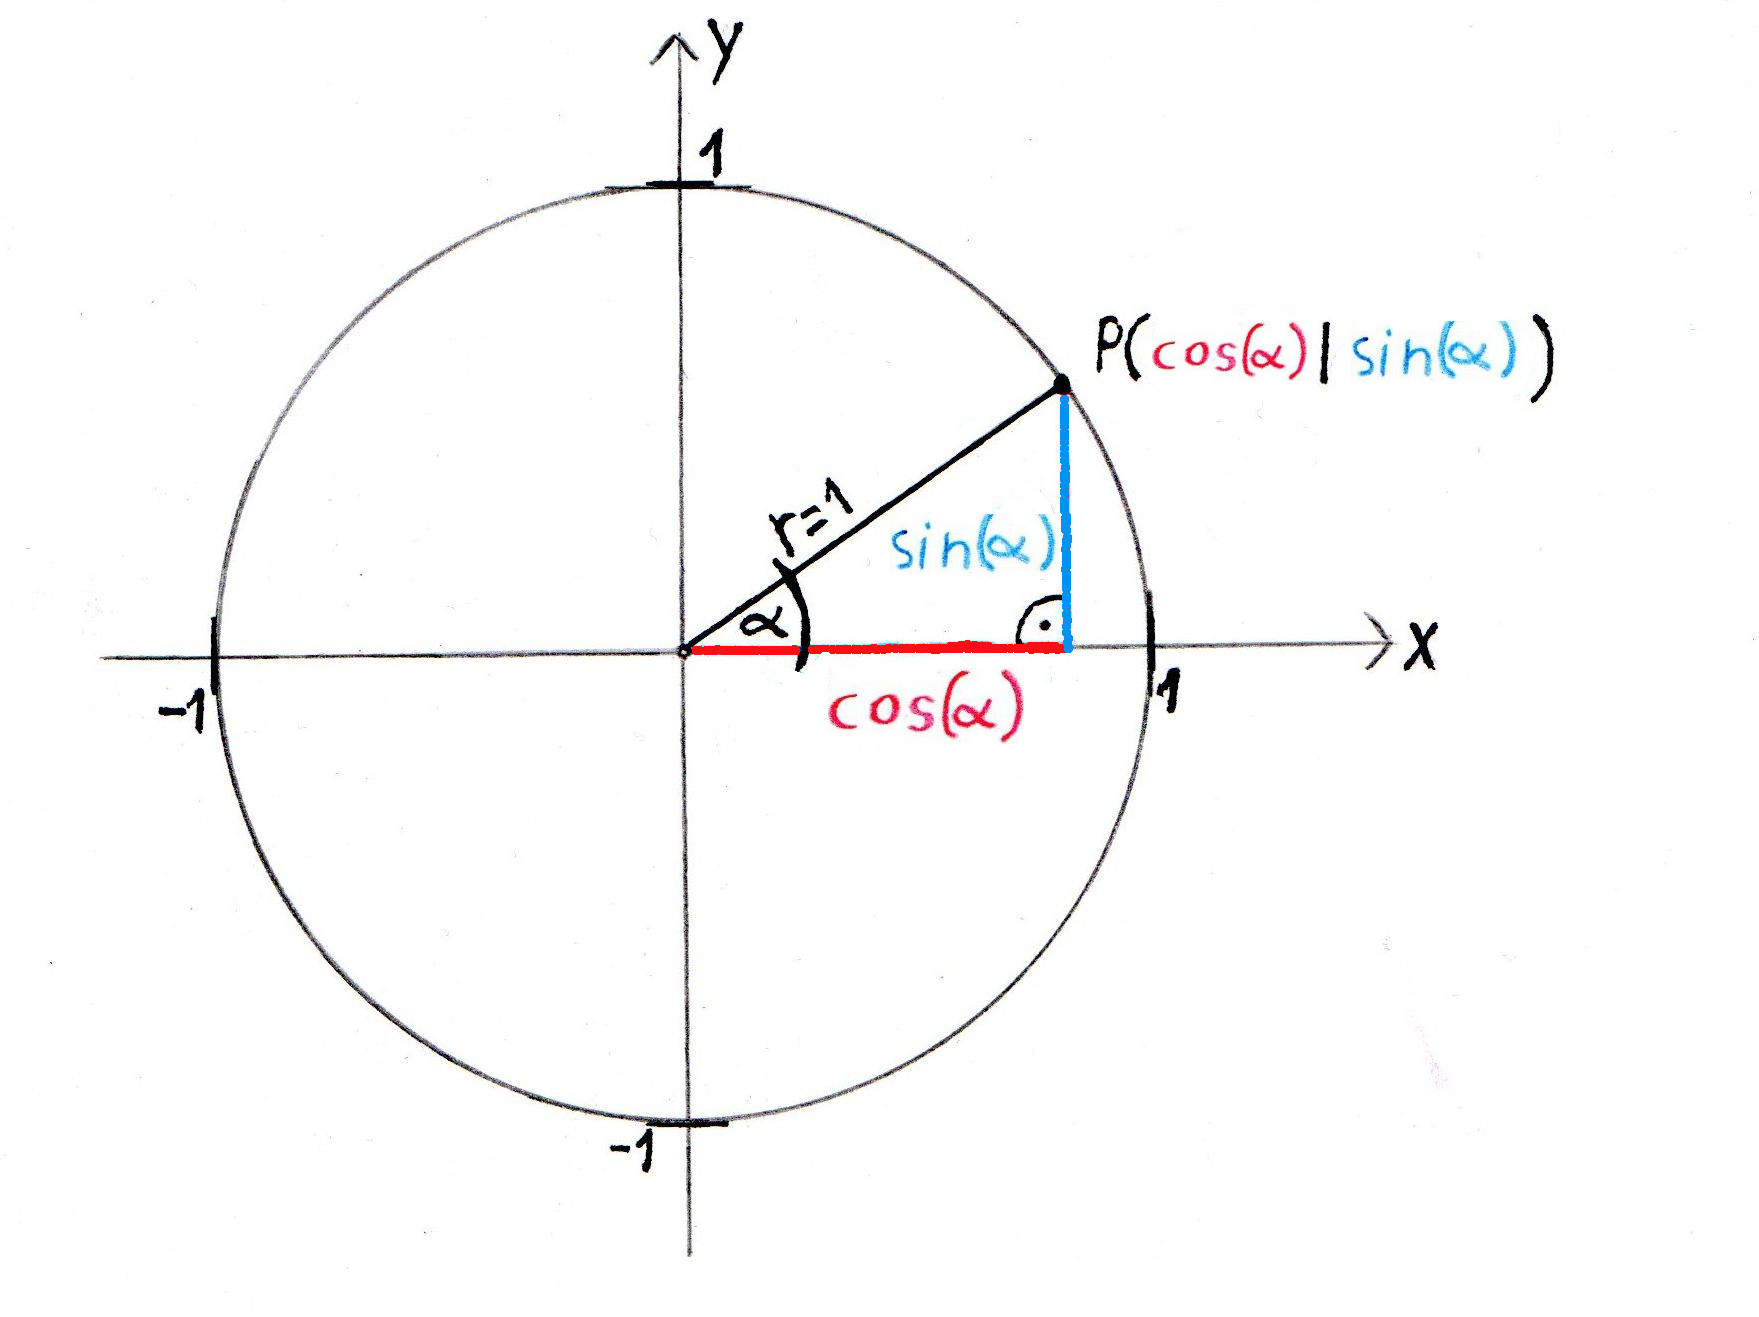
\includegraphics[scale=0.2]{Images/Einheitskreis.jpeg}
				\caption{Sinus \& Kosinus am Einheitskreis}
			\end{figure}
  
			Das Bild soll uns die Definition der trigonometrischen Funktionen erklären.
			Der Radius des Kreises ist 1. Somit wird die schräge Linie dies auch immer
			sein, egal in welchem Winkel \(\alpha\) sie zur x-Achse steht. Letzterer ist
			beliebig wählbar. Die rote Linie ist nun der Kosinus in Abhängigkeit des
			Winkels und die blaue Linie entspricht dem Sinus. Ist der Winkel 0, so ist
			unser Sinus (der y-Wert, an der die Gerade den Kreis schneidet) ebenfalls 0,
			der Kosinus (der x-Wert) entsprechend 1. Hier wird vielleicht auch
			ersichtlich, wieso sich das ganze wiederholt. Wenn nicht, empfehlen wir euch
			folgendem Link nachzugehen und durch ein wenig Ausprobieren die Funktion
			besser kennen zu lernen. Ein Dankeschön an dieser Stelle an den Autor des
			Applets Walter Fendt, welcher uns erlaubt, seine Applets zu nutzen ):
			\url{http://www.walter-fendt.de/m14d/sincostan.htm}\\
			Zuletzt noch der Tangens. Wie der Wert am Einheitskreis festgelegt ist (auch
			im Link) spielt keine große Rolle. Definiert ist er einfach als
			\(tan(x)=\frac{sin(x)}{cos(x)}\).\\
			Wir möchten noch kurz ansprechen, wie wir die trigonometrischen Funktionen in
			der Mittelstufe benutzt haben. Damit könnt ihr zum Beispiel den Winkel
			zwischen einer Funktion (bzw. deren Steigung an dem Punkt) und der x-Achse
			bestimmen. So ist bei einem rechtwinkligen Dreieck die längste Seite
			(gegenüber vom rechten Winkel) die Hypotenuse (kurz h), die Seite am Winkel
			\(\alpha\) nennt man die Ankathete (kurz a) und die andere, gegenüber des
			Winkels ist die Gegenkathete (kurz g). Damit gilt dann:
			\formel{\[sin(\alpha)=\frac{g}{h},\ cos(\alpha)=\frac{a}{h},\
			tan(\alpha)=\frac{g}{a}\]}
		\paragraph{sin, cos \& tan als Funktion}
			\todo[color=green]{Kasten für Formel hinzufügen}
			\todo[inline,color=red]{Zusammenfassung-Kasten hinzufügen}
			\todo[inline,color=red]{Signalwörter-Kasten hinzufügen}
			Wie wir schon zuvor angekündigt hatten, ist bei diesen Funktionen viel zu
			beachten. Wir möchten als Beispiel den Sinus nutzen, um euch das Prinzip zu
			erklären. Der Kosinus funktioniert aber genau so (er ist nur verschoben, wie
			wir später sehen werden). Den Tangens werden wir nur kurz andeuten, da er
			nicht oft vorkommt.\\
			Grundsätzlich stellen wir den Sinus so dar:
			\formel{\[f(x)=a\cdot sin(b(x-c))+d\]}	
			Betrachten wir zuerst die bekannten und daher einfachen Konstanten. c
			verschiebt wieder nach links oder rechts und das d nach oben oder unten.
			Verschiebt man den Kosinus um \(\frac{\pi}{2}\) nach rechts, so erhält man
			den Sinus, verschiebt man ihn um die gleiche Länge nach links, hat man den
			-sin(x) (genauer um eine \(\frac{1}{4}\) Periode, wenn diese nicht \(2 \pi\)
			ist):
			\[sin(x)=cos(x-\frac{\pi}{2})\ \&\ cos(x)=sin(x+\frac{\pi}{2})\]
			 Das a ist letztendlich wieder eine Streckung. Hier fällt einem jedoch
			 zusätzlich etwas auf: Ist das a nicht da, (wir nehmen jetzt mal an, dass die
			 Funktion nicht verschoben wurde) so haben alle Hochpunkte den Wert 1 und
			 alle Tiefpunkte den Wert -1. Mit a sind alle Werte zwischen a und -a.
			 Selbiges bei einem verschobenen Graphen herauszufinden, ist etwas komplexer.
			 Wir nehmen einfach den höchsten Punkt und ziehen ihn vom niedrigsten ab und
			 teilen durch 2. Ein kleines Beispiel: Haben die Hochpunkte den Wert y=4 und
			 die Tiefpunkte den Wert y=0, so rechnen wir \(a=\frac{4-0}{2}=2\).\\
 			Nun kommen wir noch zum b. Hierzu müssen wir erst einmal wissen, was eine
 			Periode ist. Diese gibt an, wie lange es dauert, bis die Funktion wieder am
			 gleichen Status ist, wie zuvor auch schon (sie wiederholt sich ja
			 periodisch).
			 Am besten schaut man, wie der Abstand von Hochpunkt zu Hochpunkt ist. Bei
			 b=1 wären das \(2\pi\) also gerade eine Umdrehung im Einheitskreis. Durch
			 das b verändert sich aber die Periode p und zwar nach folgender Gleichung:
 			\formel{\[p=\frac{2\pi}{b}\]}
			 Die Erkenntnisse für den Sinus (und somit auch für den Kosinus) gelten auch
 			für den Tangens, mit folgender Ausnahme: Beim Tangens gibt es keine
 			Amplitude, die Streckung erfolgt also wie bei den vorherigen Funktionen.\\
 			Auch wenn wir uns hier wiederholen, aber schaut bitte unbedingt, dass euer
 			Taschenrechner mit der richtigen Winkeleinheit rechnet! Bei den
 			\textit{trigonometrischen Funktionen} nehmt am besten immer das Bogenmaß,
 			abgesehen davon, dass es sowieso meistens gebraucht wird, sehen eure Kurven
 			auf dem Taschenrechner sonst eigenartig aus und ihr lauft Gefahr, dass die
 			Rechnungen falsch sind.

%Wurzelfunktionen fliegen raus 
% \subsubsection{Wurzelfunktionen}
%Eine letzte Funktionenklasse stellt die Wurzelfunktion dar. Allgemein hat sie folgende Form:
%\[f(x)=a\sqrt[n]{b(x-c)}+d\]
%c und d Verschieben wieder, a streckt die Funktion und das b ist wieder ähnlich dem der e-Funktion (streckt also wieder in gewisser Art).


	% Zusammengesetzte Funktionen
	\section{Zusammengesetzte Funktionen}
	\todo[color=purple]{Kasten für Formel hinzufügen}
	\todo[color=purple]{Zusammenfassung-Kasten hinzufügen}
	\todo[color=purple]{Signalwörter-Kasten hinzufügen}
	Unsere Grundfunktionen können wir nun beliebig kombinieren (im Folgenden sind
	die Grundfunktionen immer als f(x) und g(x) dargestellt, die Resultierende
	nennen wir h(x)). Dieses Kapitel dient zum einen dem tieferen Verständnis der
	Materie, aber vor allem wird es uns helfen, die Ableitungs-/ \& Integral-Regeln
	zu verstehen und richtig anwenden zu können\footnote{Natürlich lassen die drei
	Möglichkeiten sich auch noch einmal miteinander kombinieren. Das werden wir im
	Kurs an einigen Beispielen sehen.}. Wenn ihr zwei Funktionen kombiniert, so
	setzt einfach die Funktion für das entsprechende f(x) oder g(x) ein.

	\subsection{Summe \& Differenzen}
		\todo[color=green]{Kasten für Formel hinzufügen}
		\todo[color=purple]{Zusammenfassung-Kasten hinzufügen}
		\todo[color=green]{Signalwörter-Kasten hinzufügen}
		Die einfachste Form ist das Addieren und Subtrahieren von zwei Funktionen.
		Dies wird vor allem nötig sein im Wahlteil, wenn man z. B. die Fläche
		berechnen will, die von zwei Funktionen eingeschlossen wird (zuerst ziehen wir
		die Funktionen voneinander ab und integrieren dann). Die Darstellung sieht
		folgendermaßen aus:
		\formel{\[h_1(x)=f(x)+g(x), \mathrm{\ bzw\ } h_2(x)=f(x)-g(x)\]}
		
		\tags{
			Summenregel
		}
	
	\subsection{Produkte \& Quotienten}
		\todo[color=green]{Kasten für Formel hinzufügen}
		\todo[color=purple]{Zusammenfassung-Kasten hinzufügen}
		\todo[color=green]{Signalwörter-Kasten hinzufügen}
		Diese Regel bei einer Funktion zu erkennen, wird uns helfen, die Faktorregel
		beim Ableiten und Integrieren anwenden zu können:
		\formel{\[h_1(x)=f(x)\cdot g(x), \mathrm{\ bzw\ } h_2(x)=\frac{f(x)}{g(x)}\]}
		
		\tags{
			Produktregel
		}

	\subsection{Verkettungen}
		\todo[color=green]{Kasten für Formel hinzufügen}
		\todo[color=purple]{Zusammenfassung-Kasten hinzufügen}
		\todo[color=green]{Signalwörter-Kasten hinzufügen}
		Eine letzte Kombination stellt die Verkettung dar. Diese werden wir beim
		Ableiten bei der Kettenregel wieder erkennen. Allgemein beschreibt man das so:
		\formel{\[h(x)=f(g(x))\]}
		Wir ersetzen also bei f(x) jedes x durch die Funktion in g(x) (alles in
		Klammern schreiben). Ein kleines Beispiel für das Verständnis: mit \(f(x)=e^x\
		\&\ g(x)=2x+3\) gilt \(h(x)=f(g(x))=e^{2x+3}\).
		
		\tags{
			Kettenregel
		}



	% Section Ableitungen (Differentialrechnung)
	\section{Ableitungen (Differentialrechnung)}
	\todo[color=red]{Kasten für Formel hinzufügen}
	\todo[color=red]{Zusammenfassung-Kasten hinzufügen}
	\todo[color=red]{Signalwörter-Kasten hinzufügen}
	Stellen wir uns zunächst einmal vor, was eine Ableitung überhaupt ist. Sie gibt
	die Steigung der Tangenten einer Funktion an jeder Stelle an. Eine Tangente
	kann man sich so Vorstellen: Nehmt ihr eine Kugel und haltet ein Buch daran, so
	stellt dieses die Tangente dar (wenn auch im Dreidimensionalen, wir brauchen
	aber nur die zweidimensionalen). Das Buch berührt die Oberfläche und liegt an
	ihr an, durchstößt sie jedoch nicht.

	% Ableitungen der Grundfunktionen
	\subsection{Ableitungen der Grundfunktionen}
	\todo[color=green]{Kasten für Formel hinzufügen}
	\todo[color=purple]{Zusammenfassung-Kasten hinzufügen}
	\todo[color=purple]{Signalwörter-Kasten hinzufügen}
	Die Herleitung für die Ableitung stammt von der mittleren Änderungsrate, welche
	die Steigung einer Sekante angibt. Dazu setzen wir einfach die zwei Punkte die
	wir haben, in folgende Funktion ein:
	\formel{\[\frac{f(x_2)-f(x_1)}{x_2-x_1}\textrm{, oder anders geschrieben }
	\frac{\Delta f(x)}{\Delta x}\]}
	Die Ableitung erfolgt dann, indem man den Abstand der Punkte
	gegen 0 laufen lässt.\\

	\(\star\) Für die ganzrationalen Funktionen, die Brüche und die
	Wurzelfunktionen gilt allgemein die Formel:
	\formel{\[f(x)=x^n\ \Rightarrow\ f'(x)=n\cdot x^{n-1}\]}
	Hier ein paar Beispiele: \(f_1(x)=x^3\ \Rightarrow\ f_1(x)=3x^2;\\
	f_2(x)=\frac{1}{x^2}=x^{-2}\ \Rightarrow\
	f_2'(x)=-2x^{-2-1}=-2x^{-3}=-\frac{2}{x^3};\\
	f_3(x)=\sqrt{x}=x^{\frac{1}{2}}\
	\Rightarrow\ f_3'(x)=\frac{1}{2}x^{-\frac{1}{2}}=\frac{1}{2\sqrt{x}}\).\\
	Konstanten ergeben abgeleitet immer 0.\\

	\(\star\) Ableitungen von exponentiellen Funktionen ergeben immer die gleiche
	Funktion wieder, jedoch mit einem Vorfaktor. Jetzt kommen wir auch endlich zum
	Sinn der eulerschen Zahl: Leitet man \(2^x\) ab, so bekommt man einen
	Vorfaktor, der kleiner ist als 1, die Ableitung von \(3^x\) einen der größer
	ist als 1. Die Ableitung von \(e^x\) hat den Vorfaktor 1, die Ableitung ist
	also gleich der eigentlichen Funktion. Wir möchten noch einmal anmerken, dass
	\(a^x=e^{ln(a)x}\) ist. Wie man das dann ableitet, wird später erklärt. Die
	Ableitung der Funktion ist jetzt also folgendermaßen:
	\formel{\[f(x)=e^x\ \Rightarrow\ f'(x)=e^x\]}

	\(\star\) Die trigonometrischen Funktionen leiten sich folgendermaßen ab:
	\formel{\[f_1(x)=sin(x)\ \Rightarrow\ f_1'(x)=cos(x)\ \&\ f_2(x)=cos(x)\
	\Rightarrow\ f_2'(x)=-sin(x)\]}
	\(\star\) Zu guter Letzt noch die Ableitung des ln:
	\formel{\[f(x)=ln(x)\ \Rightarrow\ f'(x)=\frac{1}{x}\]}
	\todo[inline,color=red]{Zusammenfassung als Bilddatei?!}

	% Summen- & Faktorregel
	\subsection{Summen- \& Faktorregel}
Diese beiden Regeln sind nicht schwer, aber sehr nützlich.\\
\(\star\) Die Summenregel besagt, wir können bei Summen einfach jeden Teil einzeln ableiten:
\[(f(x)+g(x))'=f'(x)+g'(x)\]
Dazu noch ein kurzes Beispiel: \(f'(x)=(x^2+sin(x))'=2x+cos(x)\).\\
\(\star\) Die Faktorregel sagt, wir können Zahlen, die mit der Grundfunktion multipliziert werden, einfach beim Ableiten zu ignorieren, müssen sie aber natürlich in die Ableitung mitnehmen:
\[f'(x)=(a\cdot g(x))'=a\cdot g'(x)\]
Auch hierzu ein Beispiel: \(f'(x)=(2\ sin(x))'=2\ cos(x)\)


	% Produktregel
	\subsection{Produktregel}
	\todo[color=green]{Kasten für Formel hinzufügen}
	\todo[inline,color=red]{Zusammenfassung-Kasten hinzufügen}
	\todo[inline,color=red]{Signalwörter-Kasten hinzufügen}
	Haben wir ein Produkt aus zwei unserer Grundfunktionen, so leiten wir zunächst
	die eine Funktion ab und multiplizieren sie mit der anderen (unveränderten) und
	addieren dieses Produkt zu dem Produkt der einen (unveränderten) Funktion mit
	der Ableitung der anderen. Mathematisch geschrieben\footnote{Oftmals werden die
	Funktionen auch mit v(x) und u(x) betitelt, dies tut aber nichts zur Sache, da
	wir die Funktionen ja nennen dürfen, wie wir wollen.}:
	\formel{\[h'(x)=(f(x)\cdot g(x))' = f'(x)\cdot g(x)+f(x)\cdot g'(x)\]}
	Wieder ein Beispiel für das bessere Verständnis: \(f(x)=x^2\cdot sin(x)\ =>\
	f'(x)=2x\cdot sin(x)+x^2\cdot cos(x)\)


	% Kettenregel
	\subsection{Kettenregel}
	\todo[color=green]{Kasten für Formel hinzufügen}
	\todo[inline,color=red]{Zusammenfassung-Kasten hinzufügen}
	\todo[inline,color=red]{Signalwörter-Kasten hinzufügen}
	Eine verkettete Funktion abzuleiten erfordert zuerst, dass wir eine Verkettung
	haben. Also, dass eine Grundfunktion in eine andere eingesetzt wurde. Dann gilt
	der Merksatz \emph{innere Ableitung mal äußere Ableitung}. Die innere Funktion
	in der abgeleiteten äußeren bleibt aber unverändert stehen.
	\formel{\[h(x)=f(g(x))\ \Rightarrow\ h'(x)=f'(g(x))\cdot g'(x)\]}
	Drei Beispiele hierzu: \(f_1(x)=e^{x^2}\ \Rightarrow\ f_1'(x)=e^{x^2}\cdot
	2x,\\
	f_2(x)=sin(ln(x))\ \Rightarrow\ f_2'(x)=cos(ln(x))\cdot \frac{1}{x}\).\\
	Als letztes Beispiel die Ableitung von \(3^x\): \(f_3(x)=3^x=e^{ln(3)\cdot x}\
	\Rightarrow\ f_3'(x)=ln(3)\cdot e^{ln(3)\cdot x}=ln(3)\cdot 3^x\).


	% Tangenten & Normale
	\subsection{Tangenten \& Normale}
Öfter kann es vorkommen, dass die Tangente, also die Gerade, die an der Funktion an einer Stelle anliegt, berechnet werden soll. Wie stellen wir das nun an? Am einfachsten und schnellsten ist die folgende Variante: Wir kennen die allgemeine Form einer Geraden und wie man eine Funktion verschiebt. Auch wissen wir, dass die erste Ableitung die Steigung der Funktion an dieser Stelle \(x_0\) ist. Das können wir nun anwenden, um die Tangente der Funktion am Punkt \(P(x_0|f(x_0))\) zu bestimmen. Wir setzen in unsere allgemeine Geradengleichung also die Steigung an dem Punkt ein und verschieben sie noch um die entsprechenden Werte in x- \& y -Richtung. Somit bekommen wir auch schon die Tangentengleichung:
\[t(x)=f'(x_0)\cdot (x-x_0)+f(x_0)\]
\(x_0\) ist hier eine Konstante, das x die Variable.\\
Die Normale steht senkrecht zur Tangente. Wie man die Steigung dieser berechnet, haben wir bereits gesehen. Die Verschiebung geht zum gleichen Punkt. Also ist die Normalengleichung:
\[n(x)=-\frac{1}{f'(x_0)}\cdot (x-x_0)+f(x_0)\]


	% Anwendung von Ableitungen
	\subsection{Anwendung von Ableitungen}
Ableitungen sind letztendlich ein Instrument, mit dem wir Eigenschaften von Funktionen überprüfen können oder mit denen wir Eigenschaften beschreiben und in die Mathematik übersetzen können.\\
\(\star\) Ein Beispiel ist die Änderungsrate. Die erste Ableitung spiegelt immer eine Änderungsrate der Funktion wieder, gibt also an, um wie viel sich die Funktion an einer bestimmten Stelle verändert. 
Machen wir uns das mal an einem Beispiel der Physik klar. Haben wir zum Beispiel den Ort eines Gegenstands in Abhängigkeit von der Zeit gegeben (s(t)=\ldots) und wir wollen wissen, wie sich der Ort mit der Zeit verändert, so leitet man nach der Zeit ab. Somit haben wir die Geschwindigkeit \(\frac{\Delta s}{\Delta t}\)(wobei \(\Delta\) gegen 0 geht), was eben angibt, um welche Strecke sich unser Gegenstand in einer Sekunde bewegt hat (erkennbar auch an den Einheiten ;) ). Genau so verhält sich das mit "Liter pro Zeit"\ oder allem anderen, was einen Bruch als Einheit besitzt.\\
\(\star\) Ableitungen können auch verwendet werden, um geometrische Informationen in die Sprache der Mathematik umzuwandeln. Folgendes Beispiel habt ihr vielleicht schon durchgerechnet. Man hat eine Funktion gegeben, die den Querschnitt eines Tals zwischen zwei Bergen beschreibt. Jetzt wissen wir an welchen Punkt die Sonne anfängt und der Schatten aufhört (natürlich ein Punkt auf der Funktion, also dem Querschnitt) und wir wollen wissen, in welchem Winkel die Sonne gerade zur x-Achse steht. Was wir jetzt noch (durch Überlegungen) wissen sollten ist, dass die Sonne den Berg tangential streift. Also brauchen wir die Tangente (an einer noch unbekannten Stelle). Die Steigung an der Stelle kann man dann noch als Winkel umrechnen (dazu kommen wir später noch). Wie man das ganze konkret berechnet, gehen wir im Kurs selbst durch.\\
\(\star\) Eine weitere wichtige Möglichkeit zur Anwendung von Ableitungen ist die Berechnung von Extrem- \& Wendepunkten.
\subsubsection{Extrempunkte}
Um diese zu bestimmen,  brauchen wir die ersten beiden Ableitungen. Zuerst bestimmt man die Nullstellen der ersten Ableitung, denn an Extrempunkten haben Funktionen immer die Steigung 0. Somit haben wir schon mal Stellen, an denen Extrempunkte sein \textbf{können}. Die Stellen (x-Werte) setzen wir dann in die zweite Ableitung ein, um zu schauen, ob es sich um einen Hoch- oder Tiefpunkt handelt. Haben wir in der zweiten Ableitung einen positiven Wert, so liegt ein Tiefpunkt vor. Bei einem negativem Wert haben wir einen Hochpunkt der ursprünglichen Funktion. Als Eselsbrücke kann man Smilies nehmen. Haben wir einen positiven Wert, so malen wir einen glücklichen Smilie, dessen Mund einen Tiefpunkt bildet. Bei einem negativen Wert malen wir einen traurigen Smilie, dessen Mund einen Hochpunkt besitzt. Weiter muss man den Punkt berechnen, an dem der Extremwert ist. Die Stelle \(x_0\) kennen wir ja bereits und müssen diese nun in die eigentliche Funktion f(x) einsetzen. Somit bekommen wir den Extrempunkt \(P(x_0|f(x_0))\).\\
Ein Problem ist es, wenn die zweite Ableitung 0 ergibt. Dann setzt man einfach in die erste Ableitung ein x kleiner als die Stelle ein und ein x, ein bisschen größer als diese Stelle, um die Steigung links und rechts von dem Extrempunkt zu ermitteln. \\
Ist die Steigung erst positiv, dann negativ, so haben wir einen Hochpunkt, umgekehrt einen Tiefpunkt. Sind beide Seiten positiv oder beide negativ, so haben wir einen Sattelpunkt. Diese Variante ist mit Nachdenken verbunden und man muss verstanden haben, wieso das so ist.\\
Noch ein kurzes Beispiel zu Extrempunktberechnungen im allgemeinen: Untersuchen wir die Funktion \(f(x)=\frac{1}{4}x^4+x^2\) auf Extremstellen. Die ersten zwei Ableitungen sind \(f'(x)=x^3+2x,\ f''(x)=3x^2+2\). Eine der potentiellen Extremstellen ist 0 (denn f'(0)=0). Eingesetzt in die zweite Ableitung ergibt f''(0)=2>0, also haben wir einen Tiefpunkt vorliegen.
\subsubsection{Wendepunkte}
Wendestellen / -punkte berechnet man ganz ähnlich wie Extrempunkte. Allerdings berechnen wir hier die Extrempunkte der ersten Ableitung. Die Nullstelle der zweiten Ableitung, eingesetzt in die dritte Ableitung, gibt uns die Richtungsänderung. Ändert sich die Kurve der Funktion von links nach rechts, haben wir bei der dritten Ableitung einen negativen Wert (\(f'''(x_w)<0)\), also der Hochpunkt der ersten Ableitung) und umgekehrt.
\subsubsection{Winkel zwischen Funktionen und Achsen}
\(\star\) Um den Winkel zwischen einer Funktion und der x-Achse zu berechnen, brauchen wir zunächst die erste Ableitung, um so die Steigung an der entsprechenden Stelle zu bekommen. Mit einer Skizze kann man sich nun herleiten, wie man den Winkel berechnet. Zeichnen wir eine Gerade mit entsprechender Steigung inklusive Steigungsdreieck (wobei wir 1 nach rechts und \(f'(x_0)\) nach oben, bzw. unten gehen), so haben wir ein rechtwinkliges Dreieck mit bekannten Katheten und können mit dem Tangens entsprechend den Winkel berechnen:
\[\alpha = tan^{-1}(f'(x_0))\]
\(\star\) Den Winkel zwischen zwei Funktionen an einer Stelle (im Normalfall der Schnittpunkt der Funktionen) berechnet man, indem zuerst wie oben beschrieben, die Winkel der Funktionen mit der x-Achse berechnet werden (aber natürlich an der entsprechenden Stelle \(x_0\)). Die beiden Winkel werden dann voneinander abgezogen, um den Schnittwinkel zu bekommen.\\
Beachtet auch, dass es immer zwei Schnittwinkel gibt, zumeist einen größeren und einen kleineren und immer ist  der kleinere der Gesuchte ! Ist euer berechneter Winkel größer als \(90^\circ\), so zieht ihr diesen einfach von \(180^\circ\) ab.



	% Section Integralrechnung
	\section{Integralrechnung}
	\todo[color=green]{Kasten für Formel hinzufügen}
	\todo[color=purple]{Zusammenfassung-Kasten hinzufügen}
	\todo[color=green]{Signalwörter-Kasten hinzufügen}
	Grundsätzlich sind Integrale die Umkehrung der Ableitung. Integrieren wir also
	eine Ableitung, (oder leiten ein Integral ab) so haben wir wieder unsere
	ursprüngliche Funktion. Mathematisch lässt sich das folgendermaßen
	darstellen\footnote{Diese Erkenntnis können wir auch nutzen, um unsere
	Integrale zu überprüfen. Wir leiten das Integral einfach ab und schauen dann,
	ob wieder die ursprüngliche Funktion raus kommt.}:
	\formel{\[\int f'(x)\ dx=f(x)\]}
	Mit Integralen macht man hauptsächlich zwei Dinge. Haben wir eine bestimmte
	Funktion, so berechnet man mit dem Integral den Flächeninhalt zwischen ihrem
	Schaubild und der x-Achse. Das kann man natürlich einfach so nutzen, um die
	Fläche dazwischen explizit auszurechnen, auch zwischen zwei Funktionen. Die
	Relation, die wir oben gesehen haben, können wir auch nutzen. Haben wir eine
	Änderungsrate (z. B. eine Geschwindigkeit) so gibt das Integral die
	tatsächliche Änderung (oft auch der Bestand genannt, z. B. die zurückgelegte
	Strecke) an.
	
	\tags{Flächeninhalt, Stammfunktion, Bestandsmenge}

	% Unbestimmte Integrale/Stammfunktionen der Grundfunktionen
	\subsection{Unbestimmte Integrale/Stammfunktionen der Grundfunktionen}
	\todo[color=red]{Kasten für Formel hinzufügen}
	\todo[color=red]{Zusammenfassung-Kasten hinzufügen}
	\todo[color=red]{Signalwörter-Kasten hinzufügen}
	Hier können wir eigentlich die Tabelle der Ableitungen nehmen, nur dass wir sie
	von rechts nach links lesen (also wir schauen, was f'(x) ist und das f(x) ist
	dann unser Integral). Deshalb werden wir uns sparen, hier alle noch einmal
	aufzulisten.\\
	Bei den ganzrationalen, Wurzel- \& Bruchfunktionen mag das vielleicht nicht
	ganz so ersichtlich sein:
	\[f(x)=x^n\ \Rightarrow\ F(x)=\int f(x)\ dx=\frac{1}{n+1}\cdot x^{n+1}+c\]
	Dazu zwei Beispiele:\(f_1(x)=x^4\ \Rightarrow\ F_1(x)=\int f_1(x)\
	dx=\frac{1}{5}\cdot x^5+c;\\
	 f_2(x)=\sqrt{x}=x^\frac{1}{2}\ \Rightarrow\ F_2(x)=\int f_2(x)\
	 dx=\frac{2}{3}\cdot x^{\frac{3}{2}}+c=\frac{2}{3}\cdot \sqrt{x^3}+c\).\\ \\
	Wichtig ist noch eine Ausnahme:
	\[f(x)=\frac{1}{x}\ \Rightarrow\ \int f(x)\ dx=ln(x)+c\]


	% Bestimmte Integrale
	\subsection{Bestimmte Integrale}
	\todo[color=purple]{Zusammenfassung-Kasten hinzufügen}
	Bestimmte Integrale geben explizit die Fläche zwischen einer Funktion und der
	x-Achse in einem Intervall an. Man erhält also eine Zahl, wenn man dieses
	berechnet. Zuerst sucht man die Stammfunktion F(x) und setzt in diese die obere
	Grenze ein. Anschließend zieht man von diesem Wert den Wert der Stammfunktion,
	mit der unteren Grenze eingesetzt, ab. Der neue Wert ist unser Ergebnis. Das
	ganze sieht dann allgemein wie folgt aus:
	\formel{\[\int\limits_a^b f(x) \ dx=F(b)-F(a)\]}
	
	\tags{Flächeninhalt zwischen x-Achse und Funktion, Bestand}

	% Summen- & Faktorregel
	\subsection{Summen- \& Faktorregel}
Ganz synchron zu der Summenregel beim Ableiten dürfen wir die einzelnen Summen einzeln integrieren:
\[\int (f(x)+g(x))\ dx=\int f(x)\ dx+\int g(x)\ dx\]
Auch die Faktorregel ist gleich. Eine konstante (z. B. eine Zahl) als Faktor vor der Funktion wird einfach bei der Stammfunktion dazugeschrieben, ohne sie weiter zu beachten:
\[\int c\cdot f(x)\ dx=c\cdot \int f(x)\ dx\]


	% Lineare Substitution ('Kettenregel')
	\subsection{Lineare Substitution ('Kettenregel')}
	\todo[color=purple]{Kasten für Formel hinzufügen}
	\todo[color=purple]{Zusammenfassung-Kasten hinzufügen}
	\todo[color=purple]{Signalwörter-Kasten hinzufügen}
	Verkettungen zu integrieren ist leider um einiges komplizierter, als beim
	Ableiten. Ihr habt aber Glück, dass im Abitur lediglich die lineare
	Substitution benutzt wird, sprich es gibt nur eine lineare Funktion (z. B.
	g(x)=f(3x +2)), die in einer anderen steckt. Haben wir eine solche Funktion
	vorliegen, so müssen wir lediglich zu dem Integral der äußeren Funktion, die
	Zahl vor dem x (hier die 3) als Kehrwert dazu multiplizieren. Wir werden hier
	lediglich ein Beispiel zeigen, allerdings gilt das bei allen Funktionen
	genauso:
	\[f(x)=sin(3x+4)\ =>\ \int f(x)\ dx=-\frac{1}{3}\cdot cos(3x+4)\]


	% Anwendungen des Integrals
	\subsection{Anwendungen des Integrals}
	\todo[color=red]{Kasten für Formel hinzufügen}
	\todo[color=red]{Zusammenfassung-Kasten hinzufügen}
	\todo[color=red]{Signalwörter-Kasten hinzufügen}
	Hier möchten wir noch einmal darauf eingehen, wie man die Integrale verwenden
	kann. Dabei gehen wir auf drei Arten ein:

	\subsubsection{Flächeninhalte}
		\todo[color=red]{Kasten für Formel hinzufügen}
		\todo[color=red]{Zusammenfassung-Kasten hinzufügen}
		\todo[color=red]{Signalwörter-Kasten hinzufügen}
		Da man das Integral über die Flächeninhalte definieren kann, ist es natürlich
		auch logisch, dass man damit Flächeninhalte berechnen kann. Und zwar immer
		den Flächeninhalt zwischen der Funktion und der x-Achse. Allerdings können diese Flächeninhalte Vorzeichen haben und sich somit auch gegenseitig aufheben. Das wollen wir dann allerdings nicht. Das Problem löst man ganz einfach, indem man die Nullstellen findet und immer von Nullstelle zu Nullstelle integriert und von den einzelnen Integralen den Betrag nimmt, also wenn nötig, das Vorzeichen ändert. Ein Beispiel hierzu:
		\[f(x)=x^2-4\textrm{, mit den Nullstellen }x_0=\pm2\ =>\ \int\limits_0^4
		|f(x)|\ dx=|\int\limits_0^2 f(x)\ dx|+|\int\limits_2^4 f(x)\ dx|\]
		Wollen wir den Flächeninhalt zwischen zwei Funktionen, so ziehen wir einfach
		die eine Funktion von der anderen ab und Integrieren dann (also wir Integrieren dann h(x)=f(x)-g(x)).

	\subsubsection{Rekonstruierter Bestand}
		\todo[color=red]{Kasten für Formel hinzufügen}
		\todo[color=red]{Zusammenfassung-Kasten hinzufügen}
		\todo[color=red]{Signalwörter-Kasten hinzufügen}
		Wie schon bei den Anwendungsaufgaben für Ableitungen gezeigt, kann man
		jegliche Form von Geschwindigkeiten als Ableitung angeben. Haben wir also nun
		eine Geschwindigkeit als Funktion angegeben und Integrieren diese, so können
		wir den eigentlichen Bestand rekonstruieren. Oder zu deutsch, wir schauen,
		welche Strecke bis zu diesem Zeitpunkt zurückgelegt wurde (bzw. wie viel Liter
		eingelassen wurden oder allgemein immer der obere Teil der Einheit). Hier wird
		dann der Teil angegeben, der vom Anfangswert dazu kam oder weg ging. Hier
		müsst ihr aber beachten, dass ihr das Integral nicht aufsplitten dürft, wie
		beim Berechnen von Flächeninhalten. Der negative Teil wird dann zwar
		mitberechnet, dass macht bei näherer Überlegung aber auch Sinn. Ist die
		Geschwindigkeit negativ, so führt das Fahrzeug auch in negative Richtung.
		Genau das sagt uns der negative 'Flächeninhalt'.\\
		Hierzu passiert es bei schwereren Aufgaben, dass man Funktionen kombinieren
		muss. Beispielsweise soll der Abstand zwischen zwei sich unterschiedlich
		bewegenden Fahrzeugen untersucht werden, deren Geschwindigkeiten wir kennen.
		Am Einfachsten ist es, die Geschwindigkeiten voneinander abzuziehen, wodurch
		wir eine neue Funktion erhalten und diese dann integrieren können. Das ist so,
		weil wir die relative Geschwindigkeit betrachten (ähnlich wird auch der
		Flächeninhalt zwischen zwei Schaubildern betrachtet).

	\subsubsection{Mittelwert}
		\todo[color=red]{Kasten für Formel hinzufügen}
		\todo[color=red]{Zusammenfassung-Kasten hinzufügen}
		\todo[color=red]{Signalwörter-Kasten hinzufügen}
		Mit dem Integral können wir auch den Mittelwert \(\overline{m}\) der
		eigentlichen Funktion f(x) in einem Intervall von a nach b berechnen. Das
		sieht dann folgendermaßen aus:
		\[\overline{m}=\frac{1}{b-a}\cdot \int\limits_a^b f(x)\]



	% Section Rechnen mit Funktionen
	\section{Rechnen mit Funktionen}
	Abschließend mit der Analysis wollen wir an dieser Stelle grundsätzliche Dinge
	besprechen, für die wir mittlerweile das Werkzeug haben.

	% Aufstellen von Funktionen
	\subsection{Aufstellen von Funktionen}
\todo[color=red]{Kasten für Formel hinzufügen}
\todo[color=red]{Zusammenfassung-Kasten hinzufügen}
\todo[color=red]{Signalwörter-Kasten hinzufügen}
Es kommt öfter vor, dass man Funktionen selbst aufstellen muss. Dazu sollte man sich zuerst überlegen, welche Art von Grundfunktion man dazu benötigt. Das zu erkennen ist Übungssache, meist steht jedoch dabei, welche ihr verwenden sollt. Je nach Angaben kann man einfach Verschiebungen und Streckungen an ihnen vollziehen. Trotzdem wollen wir das nochmals kurz durchgehen.\\
\(\star\) Haben wir einen Vorgang, der sich in einer bestimmten Zeit verdoppelt, halbiert oder ähnliches, so können wir dies als e-Funktion darstellen.\\
\(\star\) Bei einem sich wiederholenden Vorgang handelt es sich um eine Sinus- oder Kosinusfunktion. Diese sind gesondert zu beachten, wenn man diese nicht mit dem Taschenrechner löst, da man hier Amplitude und Periode ermittelt und diese dann einfach einsetzt.\\
\(\star\) Bei den anderen Funktionen kann man dies meist auch auf folgende Art lösen (manchmal auch nur): Zuerst einmal stellen wir Bedingungen auf. Das bedeutet, wir setzen in unsere Funktion alle Daten ein, die wir kennen (z. B. wenn wir den Punkt (1|2) kennen, so setzen wir f(1)=2 ein und einen Extrempunkt an der Stelle 5 wird mit f'(5)=0 angegeben). Die Faktoren, die wir nicht kennen, lassen wir einfach entsprechend stehen und haben dann ein Gleichungssystem, dass wir lösen können. Grundsätzlich gilt, man braucht mindestens so viele Informationen, wie man Variablen hat. Bei einer ganzrationalen Funktion mit dem Grad n haben wir immer n + 1 Unbekannte. Haben wir zum Beispiel eine ganzrationale Funktion mit dem Grad 3, so haben wir 4 Faktoren und um diese zu lösen, benötigen wir mindestens 4 Bedingungen.


	% Kurvendiskussion
	\subsection{Kurvendiskussion}
Sollt ihr eine Kurvendiskussion durchführen, so wäre folgende Reihenfolge sinnvoll\footnote{Die Reihenfolge bleibt im großen und ganzen euch überlassen. Es empfiehlt sich aber, sich an eine Reihenfolge zu halten, damit ihr nichts vergesst.}:\\
1. Definitionsmenge\\
2. Punkt- \& Achsensymetrie\\
3. Verhalten für \(x \rightarrow \pm \infty\)\\
4. Polstellen\\
5. Schnittpunkte mit y-Achse und x-Achse\\
6. Extrem- \& Sattelpunkte\\
7. Wendepunkte\\
8. Monotonie\\
9. Zeichnen der Funktion\\ \\
Wie man die Punkte abarbeitet, werden wir nun noch einmal einzeln durchgehen. Im Eigentlichen sind das aber lediglich die Anwendungen dessen, was wir bisher gelernt haben.
\subsubsection{Definitionsmenge}
Das wurde zwar schon angesprochen, wir wiederholen es aber an diesem Punkt noch einmal. Der Definitionsbereich umfasst jede Zahl, die ihr einsetzen dürft (meistens alle reellen Zahlen; es gibt jedoch drei Ausnahmen):\\
\(\star\) Im Nenner eines \underline{Bruchs} darf niemals eine 0 stehen, hier wäre die Funktion an dieser Stelle nicht definiert. Kommen in einer Funktion Brüche vor, so ermittelt ihr einfach die Nullstellen des Nenners. Das sind dann die Zahlen die nicht eingesetzt werden dürfen. Dargestellt würde das so \(\mathbb D = x \in \mathbb R \backslash\{x_0,\ x_1, \ldots \}\).\\
\(\star\) In \underline{geraden Wurzeln} (also die 2-te, 4-te, 8-te \ldots Wurzel) dürfen keine negativen Zahlen stehen, da der Wertebereich der Normalparabel lediglich im positiven definiert ist. Hierzu ist es hilfreich, sich wieder die Nullstellen zu suchen und Zahlen zwischen zwei Nullstellen einzusetzen, bzw. links oder rechts von ihnen. Jeder Bereich zwischen den Nullstellen des Terms in der Wurzel der negativ ist, fällt dann aus der Definitionsmenge raus.\\
\(\star\) \underline{Logarithmusfunktionen} sind ähnlich zu behandeln wie die Wurzelfunktionen, nur dass hier auch die 'Nullstellen' im ln wegfallen.
\subsubsection{Punkt- / Achsensymmetrie}
Um eine Symetrie zu untersuchen, setzt ihr einfach für jedes x ein (-x) ein (bitte auch in Klammern!) und schaut, wie sich die Funktion im ganzen verändert.\\
Eine (y-)Achsensymetrie erkennt man daran, dass wir die gleiche Funktion nach Einsetzen des (-x) wieder erhalten. Dies ist zum Beispiel bei ganzrationalen Funktionen, welche nur gerade Hochzahlen besitzen, der Fall. Auch der Kosinus ist Achsensymetrisch, wenn er nicht nach links oder rechts verschoben wurde.
\[f(-x)=f(x),\mathrm{\ Bsp.\ } f(-x)=(-x)^2+1=x^2+1=f(x)\]
Eine Punktsymetrie am Ursprung liegt vor, wenn wir beim Einsetzen von (-x) die selbe Funktion wieder erhalten, nur dass sie komplett mit -1 multipliziert wurde. Dies ist der Fall bei ganzrationalen Funktionen mit nur ungeraden Exponenten und dem Sinus zum Beispiel. So gilt:
\[f(-x)=-f(x),\mathrm{\ Bsp.\ } f(-x)=(-x)^3+sin(-x)=-x^3-sin(x)=-(x^3+sin(x))\]
\subsubsection{Verhalten gegen unendlich}
Hierbei schaut man, woher die zu untersuchende Funktion kommt und wohin sie geht.\\
\(\star\) Bei den trigonometrischen Funktionen kann man darauf keine Antwort geben, da diese ja andauernd hin und her Pendeln.\\
\(\star\) Bei ganzrationalen Funktionen kann man jedoch Aussagen machen. Man schaut hierbei lediglich auf den Grad der Funktion (also den größten Exponenten). Dieser Summand entscheidet dann alleine über das Verhalten im Unendlichen. Alle Funktionen mit geraden Exponenten kommen vom positiven Unendlichen und gehen ins positiv Unendliche, sofern natürlich der Grad nicht mit etwas negativem multipliziert wird. Dann ist natürlich genau das Gegenteil der Fall.\\
Bei einem ungeraden Grad kommt die Funktion vom minus Unendlichen und geht ins positiv Unendliche (wie \(x^3\)). Wenn der Summand, der den Grad angibt, negativ ist, dreht sich das ganze natürlich wieder um.\\
\(\star\) \(\frac{1}{x}\) geht gegen 0 in beide Richtungen.\\
\(\star\) Bei der e-Funktion geht die Funktion für \(x\rightarrow -\infty\) gegen 0, für \(x\rightarrow + \infty\) ins (positiv) Unendliche. Hier müsst ihr aber aufpassen, wenn die Funktion in der Art \(e^{-x}\) aussieht, dann vertauscht sich links und rechts entsprechend.\\
\(\star\) Bei Summen, die man betrachtet, kann man einfach das \(\infty\) (in einer Nebenrechnung) einsetzen und das Ergebnis addieren. \(\infty\) addiert mit einer Zahl gibt trotzdem \(\infty\).\\
\(\star\) Bei Produkten von Funktionen gibt es eine Art Rangfolge. \(e^x\) dominiert das Ergebnis immer, bei reinen ganzrationalen Funktionen dominiert der höchste Grad.

%gebrochenrationale fliegen raus
%\(\star\) Bei gebrochenrationalen Funktionen muss man zwischen 3 Arten unterscheiden. Selbige kann man als Bruch zwischen 2 ganzrationalen Funktionen darstellen (zur Erinnerung: \(h(x)=\frac{f(x)}{g(x)}\)). Nun unterscheidet man einfach, welcher Grad größer ist, der der oberen Funktion oder der der unteren.\\
%Hat die obere Funktion den größeren Grad, so betrachtet man einfach diese, wie oben beschrieben und muss nichts weiter beachten.\\
%Ist der Grad der Funktion im Nenner größer, so geht die Funktion immer gegen 0 (wie z. B. auch \(\frac{1}{x}\)).\\
%Zu guter Letzt kann es natürlich auch Vorkommen, dass beide Grade gleich groß sind. Dann klammert man nach dem Distributivgesetz das x mit der höchsten Potenz aus, wodurch man das Verhalten gegen unendlich leicht ablesen kann. Leicht erkennt man das an folgendem Beispiel:
%\[f(x)=\frac{2x^3+x}{3x^3+2}=\frac{x^3}{x^3}\cdot\frac{2+\frac{1}{x^2}}{3+\frac{2}{x^3}}\]
%Letztendlich geht unsere Funktion also gegen \(\frac{2}{3}\) (das \(x^3\) kürzt sich ja weg). Es fällt letztendlich auf, dass immer die Zahlen vor den höchsten Potenzen (hier das \(x^3\)) den Grenzwert anzeigen.

\subsubsection{Polstellen}
Polstellen treten bei Definitionslücken (zum Beispiel bei gebrochenrationalen Funktionen) auf. Hier ist anzugeben, ob f(x) an dieser Stelle gegen \(+\infty\ oder\ -\infty\) geht. Am einfachsten zu erkennen ist das indem man bei der Ableitung kurz vor und hinter der Polstelle (also entsprechendes x in der Nähe) einsetzt. Ist die Ableitung dort positiv, so gilt \(f(x)\rightarrow + \infty\) an dieser Stelle.
\subsubsection{Schnittpunkte mit den Achsen}
\(\star\) Zuerst ermittelt man den Schnittpunkt mit der y-Achse. Hierzu setzen wir f(0) und haben so den y-Achsenabschnitt. Das macht von daher Sinn, da sich an der Stelle x=0 die y-Achse befindet. Der Punkt ist dann S(0|f(0)).\\
\(\star\) Den Schnittpunkt oder die Schnittpunkte mit der x-Achse nennt man auch Nullstellen, da wir an diesen Stellen (x-Werten) den Funktionswert 0 haben. Daher können wir mit Kommentar lediglich die x-Stellen angeben oder die Punkte. Wenn nicht anders verlangt, bleibt das euch überlassen\footnote{Achtet dann aber darauf, was ihr dazu schreibt! Wenn ihr von Nullstellen redet, dürft ihr keine Punkte angeben und umgekehrt. Je nach dem, wie streng eure Korrektoren sind, kann das als Fehler gewertet werden, vermeidet das also}. Um Nullstellen zu ermitteln gilt allgemein f(x)=0. Die Lösungen der Gleichung für x sind dann diese\footnote{Im Wahlteil habt ihr ja den CAS und könnt dann einfach mit solve(...) das ganze auflösen.}. Gehen wir nun das ermitteln der Nullstellen bei den verschiedenen Funktionstypen durch:\\
\(\star\) Bei ganzrationalen Brüchen klammert man zuerst nach dem Distributivgesetz so viele x wie möglich aus (ohne das Brüche entstehen). Ist dies möglich, so hat die Funktion eine Nullstelle bei x=0, da der gesamte Term 0 wird, wenn einer der Faktoren (hier das alleinstehende x) 0 wird. Da bei euch die Polynomdivision entfällt, bleibt dann im Faktor eine quadratische oder sogar lineare Funktion. Wann diese 0 wird, ist einfach in einer neuen Gleichung zu ermitteln. Gebrochenrationale werden immer dann 0, wenn der Zähler 0 wird, wodurch es sich auf das Problem einer ganzrationalen Funktion reduziert. Ihr müsst dann lediglich darauf schauen, dass die Nullstelle im Definitionsbereich liegt.\\
\(\star\) Bei trigonometrischen Funktionen ist das im allgemeinen nicht so einfach, im Pflichtteil werden im Normalfall aber nur 3 einfache Fälle vorkommen =). Sind sie nicht in y-Richtung verschoben, so müsst ihr lediglich eine angeben, in der Sinus oder Kosinus 0 ist und dann mit dem Term im Sinus / Kosinus damit gleichsetzen und bekommt so die Nullstelle:
\[f(x)=sin(x+\frac{\pi}{2}),\mathrm{\ so\ sind\ Nullstellen:\ }x_0=\frac{\pi}{2}+k\cdot \frac{\pi}{2}\]
Das \(k\cdot \frac{\pi}{2}\) zeigt an, dass sich jede viertel Periode eine weitere Nullstelle befindet (je nach Periode muss also der Faktor entsprechend verändert werden). Sollte die Funktion in y-Richtung um die Amplitude verschoben sein, so muss man entsprechend Hoch- / Tiefpunkt berechnen und angeben. Hier befindet sich um exakt eine Periode verschoben, eine neue Nullstelle. Sollte die Verschiebung größer als die Amplitude sein, so gibt es keine Nullstellen.
\subsubsection{Extrem- / Sattelpunkte \& Wendepunkte}
Wie man diese berechnet, haben wir ja bereits erläutert :)
\subsubsection{Monotonie}
Monotonie ist ein anderer wichtiger Teil für die Kurvendiskussion. Dazu schaut man sich einfach die erste Ableitung an. Alle Extrem- und Polstellen können wir dann als Grenzen für die Intervalle nehmen, die wir im folgenden betrachten. Ob die Intervalle monoton steigen oder fallen, bestimmt man dann, indem man eine beliebige Stelle im Intervall in die Ableitung einsetzt. Ist sie positiv, so ist die Funktion in jenem Intervall monoton steigend; ist sie negativ, dann monoton fallend. Ein Beispiel: bei der Funktion \(f(x)=x^2\) würde man entsprechend aufschreiben: Für \(-\infty \le x \le 0\) ist f(x) monoton fallend, für \(0\le x\le \infty\) monoton steigend.
\subsubsection{Zeichnen der Funktion}
Zu guter Letzt kann man die Punkte in das Schaubild eintragen und anhand der anderen Informationen der Kurvendiskussion den Graphen selbst recht genau bestimmen.

\subsection{Funktionsscharen}
Funktionsscharen bereiten oft Probleme. Jedoch sind sie nicht wesentlich komplizierter als die üblichen Funktionen, wenn man sich klar macht, wie sie aufgebaut sind. Man behandelt sie ganz einfach wie alle anderen Funktionen und behandelt den \textit{Parameter wie eine Zahl}. Denn eigentlich ist sie das auch, nur kennen wir jene Zahl nicht und ersetzen sie durch einen Buchstaben. So bekommen wir oftmals Punkte oder Stellen in Abhängigkeit der Parameter. \\
Ein Beispiel: Wollen wir die Extremstelle der Funktion \(f_a(x)=x^2-ax+4\) bestimmen, so leiten wir zunächst nach der Variablen ab (\(f_a'(x)=2x-a \ \& \ f_a''(x)=2\)). Nun setzen wir die erste Ableitung 0 und erhalten so eine Extremstelle bei \(x_0=\frac{a}{2}\). Eingesetzt in die zweite Ableitung, erhalten wir immer eine positive Zahl. Also haben wir immer einen Tiefpunkt, unabhängig von a. Eingesetzt in die Ursprungsfunktion erhalten wir so für alle a den Tiefpunkt \(T(\frac{a}{2}|-\frac{a^2}{4}+4)\).\\
Das einzige was hier als Neues hinzukommt ist, dass ein gemeinsamer Schnittpunkt für alle Funktionen der Funktionsschar gesucht werden soll (was aber nicht zwangsweise der Fall sein muss!). Hierzu setzt man für den Parameter 2 unterschiedliche 'Zahlen' ein (nicht zu wörtlich nehmen!), die wir nicht kennen und deshalb 2 verschiedene Buchstaben dafür nehmen.  Angenommen, wir haben \(f_a(x)=a^x\), dann setzen wir diese mit einer anderen Funktion der Schar gleich (\(f_a(x)=f_b(x)\)). Wie wir an folgender Rechnung sehen, wird, unabhängig vom Paramenter, jede Funktion durch den Punkt P(0|1) gehen. Wieso ist das so?
\[a^x=b^x\ \Rightarrow\ e^{x\ ln(a)}=e^{x\ ln(b)} \ |ln\ \Rightarrow\ x\ ln(a)=x\ ln(b)\ \Rightarrow\ x\cdot (ln(a)-ln(b))=0\]
Einem ähnlichem Schema folgen alle Aufgaben dieser Art.

\subsection{Beschränktes Wachstum \& Differentialgleichung}
Für ein beschränktes Wachstum wird die e-Funktion (\(f(x)=a\cdot e^{b(-x-c)}+d\)) benutzt. Unser b ist dann negativ, sodass der Wert der Funktion immer kleiner wird und sich einem Wert annähert und zwar unserer Verschiebung in y-Richtung d (Schranke genannt). Nun ist zu prüfen, ob wir uns der Grenze von oben (beschränkte Schrumpfung) oder von unten (beschränktes Wachstum) nähern. Bei letzterem müssen wir ein entsprechendes negatives a einsetzen. Am Besten könnt ihr das mit einer Skizze herleiten.\\
Schauen wir uns noch kurz an, was Differentialgleichungen sind. In einer solchen Gleichung sind sowohl die eigentliche Funktion als auch deren Ableitung vorhanden (meist ohne diese selbst zu kennen). Diese aufzulösen ist nicht so leicht. Da ihr diese aber nur beim Thema beschränktes Wachstum benutzt, lässt sich das Ganze auf eine einfache Art reduzieren. Findet ihr eine Differentialgleichung vor, die (zumindest durch umformen) wie folgt aussieht
\[f'(x)=k\cdot (S-f(x)),\]
so sind Funktion und Ableitung:
\[f(x)=S+a\cdot e^{-kx},\ f'(x)=-ake^{-kx}\]
Ihr könnt also entsprechend die Variablen einsetzen, um eure Funktion zu finden. Um zu schauen, ob die Differentialgleichung stimmt, setzt einfach die Funktionen und Ableitung entsprechend oben ein.



	
	% Analytische Geometrie (Vektoren)
	\chapter{Analytische Geometrie (Vektoren)}
	Der Zweite Teil des Mathe-Abis bezieht sich auf das Rechnen mit Vektoren.
	Unsere Elemente mit denen wir rechnen, sind nun keine Zahlen (diese werden
	Skalare genannt) mehr, sondern Vektoren. Mit ihnen lassen sich dreidimensionale
	Räume leichter darstellen und berechnen\footnote{Tatsächlich gibt es auch mehr
	Dimensionen die man damit berechnen kann, einige Theorien beschäftigen sich
	sogar mit unendlich-dimensionalen Räumen, 3 Dimensionen reichen uns aber ;)}.

	% Section Einleitung Vektoren und Vektoren im Koordinatensystem
	\section{Einleitung Vektoren und Vektoren im Koordinatensystem}
Vektoren lernt man normalerweise erst richtig in der Oberstufe kennen, deswegen möchten wir uns zu Anfang erst einmal damit beschäftigen, was unsere neuen Elemente (also Vektoren) überhaupt sind.\\
Ein Vektor hat immer eine Richtung und eine Länge. Die verschiedenen Zahlen im Vektor geben an, wie weit der Vektor in die jeweiligen Richtungen geht. In der ersten Zeile ist dann die x-Richtung angegeben, in der zweiten die y-Richtung und der letzten Zeile die z-Richtung. Daraus ergeben sich die geforderten Längen und Richtungen. Man benennt sie normalerweise mit kleinen Buchstaben mit einem Pfeil darüber. Ein Vektor sieht dann so aus:
\[\vec{a}=\begin{pmatrix}
 a_1\\
 a_2\\
 a_3
\end{pmatrix}\]
Ein Vektor muss nicht zwingend in einem Koordinatensystem sein, meist wird dies aber der Fall sein. Es ist ähnlich wie die Koordinatensysteme, die wir bereits kennen, nur mit einer weiteren, dritten Dimension. Des weiteren legen wir fest, dass wir den Punkt P(0|0|0) Ursprung nennen, bei dem unser Start für die Vektoren liegt.

% Rechnen mit Vektoren
\subsection{Rechnen mit Vektoren}
Da die Vektoren erst neu dazu kamen, sollten wir zunächst noch einmal kurz auf die Grundrechenarten eingehen und wie diese bei Vektoren angewendet werden.
\subsubsection{Addition}
\todo[color=red]{Kasten für Formel hinzufügen}
\todo[color=red]{Zusammenfassung-Kasten hinzufügen}
\todo[color=red]{Signalwörter-Kasten hinzufügen}
Die Addition von Vektoren ist recht simpel. Wir addieren einfach die einzelnen Zeilen zueinander:
\[\vec{a}+\vec{b}=
\begin{pmatrix}
 a_1\\
 a_2\\
 a_3
\end{pmatrix}+\begin{pmatrix}
 b_1\\
 b_2\\
 b_3
\end{pmatrix}
=
\begin{pmatrix}
 a_1+b_1\\
 a_2+b_2\\
 a_3+b_3
\end{pmatrix} \]
Hier wird vielleicht auch ersichtlich, wie sich die Richtung eines Vektors zusammensetzt, wenn man ihn wie folgt umschreibt:
\[\vec{a}=
\begin{pmatrix}
 a_1\\
 a_2\\
 a_3
\end{pmatrix}=
\begin{pmatrix}
 a_1\\
 0\\
 0
\end{pmatrix} +
\begin{pmatrix}
 0\\
 a_2\\
 0
\end{pmatrix} +
\begin{pmatrix}
 0\\
 0\\
 a_3
\end{pmatrix}
\]
\subsubsection{Subtraktion}
\todo[color=red]{Kasten für Formel hinzufügen}
\todo[color=red]{Zusammenfassung-Kasten hinzufügen}
\todo[color=red]{Signalwörter-Kasten hinzufügen}
Entsprechend kann man auch zwei Vektoren voneinander abziehen. Die Subtraktion erfolgt analog zur Addition. Damit kann man auch den Vektor zwischen zwei Punkten berechnen (Ziel minus Angriff):
\[\vec{a}-\vec{b}=\begin{pmatrix}
 a_1-b_1\\
 a_2-b_2\\
 a_3-b_3
\end{pmatrix}\]
\subsubsection{skalare Faktoren}
\todo[color=red]{Kasten für Formel hinzufügen}
\todo[color=red]{Zusammenfassung-Kasten hinzufügen}
\todo[color=red]{Signalwörter-Kasten hinzufügen}
Mit einem Faktor kann man einen Vektor ums c-Fache vergrößern (oder Verkleinern), bzw. mit einem negativen Faktor die Richtung des Vektors auch um \(180^{\circ}\) drehen. Der Pfeil auf der Linie ist dann einfach auf der anderen Seite. Steht der skalare Faktor vor (oder auch hinter) dem Vektor, so ist das das Gleiche, wie wenn man das Skalar mit jeder Zeile multipliziert:
\[c\cdot \vec{a}=
\begin{pmatrix}
 c\cdot a_1\\
 c\cdot a_2\\
 c\cdot a_3
\end{pmatrix}
\]
\subsubsection{Betrag (Länge) eines Vektors}
\todo[color=red]{Kasten für Formel hinzufügen}
\todo[color=red]{Zusammenfassung-Kasten hinzufügen}
\todo[color=red]{Signalwörter-Kasten hinzufügen}
Will man die Länge eines Vektors ermitteln, so bekommt man ein Skalar mit eben dieser Länge. Man berechnet diesen, indem man den Satz des Pythagoras anwendet, allerdings für 3 Dimensionen. Das sieht dann wie folgt aus:
\[|\vec{a}|=\sqrt{a_1^2+a_2^2+a_3^2}\]
\subsubsection{Skalarprodukt}
\todo[color=red]{Kasten für Formel hinzufügen}
\todo[color=red]{Zusammenfassung-Kasten hinzufügen}
\todo[color=red]{Signalwörter-Kasten hinzufügen}
Eine Art des Produkts bei Vektoren ist das Skalarprodukt. Man multipliziert hier die Länge des Vektors, auf den anderen projektiert, mit der kompletten Länge des anderen Vektors. Wie man sich das genauer vorstellen kann, findet man im Internet oder hier in unserem Kurs ;). Man berechnet das Skalarprodukt wie folgt:
\[\vec{a}\cdot \vec{b}=a_1\cdot b_1+a_2\cdot b_2+a_3\cdot b_3\]
Somit haben wir aus zwei Vektoren ein Skalar (eine Zahl) gemacht. Welche Bedeutung dies hat sehen wir, wenn wir uns die Definition genauer anschauen. Mathematisch sieht diese wie folgt aus:
\[\vec{a}\cdot \vec{b}=|\vec{a}|\cdot |\vec{b}|\cdot cos(\varphi)\]
Mit dieser Relation kann man die Projektion erkennen und sieht auch, dass zwei orthogonale Vektoren das Skalarprodukt 0 haben. Mit dieser kann man jedoch auch den Winkel zwischen zwei Vektoren berechnen. Zwar ist dies recht leicht umzustellen, da dies aber eine wichtige Relation ist, werden wir sie noch einmal umgestellt aufschreiben\footnote{Beachtet bitte, dass es immer 2 Winkel gibt. Beide zusammen ergeben \(180^{\circ}\). Man gibt aber immer den kleineren Winkel an. Bekommt ihr also einen Winkel der größer ist als \(90^{\circ}\), so ist euer richtiger Winkel einfach: \(\alpha=180^{\circ}-\beta\)}:
\[cos(\varphi)=\frac{ | \vec{a}\cdot \vec{b} | }{|\vec{a}|\cdot |\vec{b}|}\]
\subsubsection{Kreuzprodukt}
\todo[color=red]{Kasten für Formel hinzufügen}
\todo[color=red]{Zusammenfassung-Kasten hinzufügen}
\todo[color=red]{Signalwörter-Kasten hinzufügen}
Das Kreuzprodukt ist in den meisten Klassen kein Unterrichtsstoff und wird auch nicht in der Prüfung abgefragt. Trotzdem wollen wir es hier ansprechen, da dies eine einfache Art ist, einen Normalenvektor (später bei den Ebenen) zu bestimmen und bei der Prüfung darf dieser auch verwendet werden. Das Kreuzprodukt ergibt nämlich immer einen Vektor, der zu den zwei anderen rechtwinklig steht, was der Definition eines Normalenvektors entspricht.\\
Ihn aufzustellen, mag bei den ersten Versuchen ein wenig kompliziert erscheinen. Das zu üben lohnt sich jedoch erheblich. In die erste Zeile des Kreuzprodukts (welcher ein Vektor ist) schreibt man \(a_2\cdot b_3-a_3\cdot b_2\). Nun schreibt man in den weiteren Zeilen jeweils den Buchstaben ab und addiert immer 1 auf die Indizes (aus einer 3 wird dann eine 1!):
\[\vec{a} \times \vec{b}=
\begin{pmatrix}
 a_2b_3-a_3b_2\\
 a_3b_1-a_1b_3\\
 a_1b_2-a_2b_1
\end{pmatrix}\]
Es gibt auch noch eine weitere Methode, die wir hier aber nicht schriftlich festhalten wollen. Diese besprechen wir dann im Kurs selbst.

\subsubsection{Lineare Abhängigkeit}
\todo[color=red]{Kasten für Formel hinzufügen}
\todo[color=red]{Zusammenfassung-Kasten hinzufügen}
\todo[color=red]{Signalwörter-Kasten hinzufügen}
Für das Abitur braucht ihr die Definition der linearen Abhängigkeit nicht mehr komplett zu kennen. Jedoch solltet ihr die Frage, ob zwei Vektoren linear abhängig sind, beantworten können (die Definition befasst sich auch mit mehreren Vektoren). Entscheidend wird dies, wenn wir Geraden oder Ebenen vergleichen wollen. Können wir einen Vektor durch einen anderen mit einem konstanten Faktor k multipliziert darstellen, sind diese linear abhängig. Bei 
\(k\cdot \begin{pmatrix}
 1\\
 -2\\
 4
\end{pmatrix}=\begin{pmatrix}
 -4\\
 8\\
 8
\end{pmatrix}\)
zum Beispiel überlegt man zunächst, wie man von 1 auf -4 kommt. Das gilt wenn k=-4 ist. Überprüft man das nun, so stimmt mit diesem k auch die zweite Zeile. Die dritte Zeile macht uns dann aber einen Strich durch die Rechnung, so dass diese Vektoren linear unabhängig sind (wäre die letzte Zeile -16 so würde es passen). Linear abhängig sind zwei Vektoren, wenn sich ein k finden lässt, sodass gilt:
\[\vec{a}=k\cdot \vec{b}\]



	% Section Geraden
	\section{Geraden}
Geraden können wir mithilfe von Vektoren im Raum darstellen. Schauen wir uns zunächst noch einmal an, wie wir das in der Analysis gemacht haben, um die Parallelen aufzuzeigen: f(x)=mx+c. Mit Vektoren stellt man dies ganz ähnlich dar. Zuerst hat man einen Stützvektor, der dem c ähnlich ist und ohne Variable in der Funktion steht. Der Richtungsvektor gibt, wie schon der Name sagt, die Richtung an. Vor ihm steht eine skalare Variable (meist s oder t genannt) welche sich mit unserem x vergleichen lässt. Der Richtungsvektor entspricht also der Steigung m (diese gibt ja ebenfalls die Richtung an). Somit können wir jeden Punkt \(\vec{x}\) (als Ortsvektor dargestellt) der auf unserer Geraden ist, angeben (\(\vec{a}\) ist der Stützvektor, \(\vec{b}\) der Richtungsvektor):
\[g:\ \vec{x}=\vec{a}+s\cdot \vec{b}\]
 

	% Section Ebenen
	\section{Ebenen}
Ebenso wie Geraden, können wir im 3D-Raum auch Ebenen darstellen. Dafür gibt es drei verschiedene Möglichkeiten die wir verwenden.

\subsection{Parameterform}
Um eine Ebene anhand von drei Punkten aufzustellen, ist die Parameterform am einfachsten. Sie ähnelt der Geradengleichung (ist also übersichtlicher auf dem ersten Blick) und die anderen beiden Formen lassen sich daraus leicht aufstellen (mit denen leichter weiter zu rechnen ist). Deshalb werden wir diese Form als Erstes zeigen, auch wenn man sie seltener nutzt. Zuerst haben wir wieder einen Stützvektor, wie bei der Geraden. Jedoch haben wir statt einem gleich zwei 'Richtungsvektoren', die Spannvektoren genannt werden (sie Spannen die Ebene auf). Diese berechnet man, indem man zwei Vektoren zwischen je zwei Punkten berechnet und eine skalare Variable mit ihnen multipliziert:
\[E:\ \vec{x}=\vec{a}+s\cdot \vec{b}+t\cdot \vec{c}\]

\subsection{Normalenform}
Mit der Normalenform können wir leichter rechnen, vergleichen und Abstände bestimmen. Die Überlegung dahinter ist ein wenig umständlicher, bei näherer Betrachtung aber nicht zwingend schwerer. Zuerst müssen wir den Normalenvektor \(\vec{n}\) finden, welcher orthogonal auf der Ebene steht. Am einfachsten und schnellsten geht das, indem wir das Kreuzprodukt der Spannvektoren berechnen, wodurch wir direkt den Normalenvektor erhalten. Eine umständlichere Variante wäre, das Skalarprodukt der Spannvektoren mit dem Normalenvektor 0 zu setzen (aufgrund der Orthogonalität) und das lineare Gleichungssystem zu lösen.\\
Nur wie kombinieren wir jetzt die Vektoren? Die Überlegung ist folgende: Wir ziehen von einem Punkt auf der Ebene den wir kennen (der Stützvektor \(\vec{a}\)), den Punkt den wir überprüfen wollen (\(\vec{x}\)) ab und bekommen so einen Vektor, von einem Punkt zum anderen. Liegt dieser auch auf der Ebene, so ist dieser rechtwinklig zum Normalenvektor (der ja zu jedem Vektor auf der Ebene orthogonal ist). Ist das nicht der Fall, liegt der Punkt irgendwie anders im Raum, aber nicht auf der Ebene. Das heißt, wenn wir den neu berechneten Vektor mit dem Normalenvektor skalar multiplizieren und der Punkt liegt auf der Ebene, so ist das Ergebnis 0:
\[E:\ (\vec{a}-\vec{x})\cdot\vec{n}=0\]
Wichtig hier zu erwähnen ist auch die hessesche Normalform. Diese unterscheidet sich lediglich durch den normierten Normalenvektor (dargestellt als \(\hat n\)). Normiert heißt hier, dass wir ihn durch die Länge teilen, er also nur noch die Länge 1 hat. Somit sieht die Hess'sche Normalenform um den Abstand d zu einem Punkt zu ermitteln, wie folgt aus:
\[E:\ (\vec{a}-\vec{x})\cdot \frac{1}{|\vec{n}|}\vec{n}=(\vec{a}-\vec{x})\cdot \hat{n}=d\]

\subsection{Koordinatenform}
An der Koordinatenform gibt es nicht viel zu verstehen. Wir müssen nur lernen, sie aufzustellen. Letztendlich ist sie aber eine Umformung der Normalenform. Hierzu brauchen wir zuerst den Normalenvektor, welchen wir mit dem erst einmal unbekannten Vektor \(\vec{x}\) skalar multiplizieren\footnote{Einfacher gesagt, setzt einfach die entsprechende Zeile des Normalenvektors zu der entsprechenden x-Zeile ein, usw.}. Auf der rechten Seite der Gleichung steht dann die Zahl w, die raus kommt, wenn wir das Skalarprodukt einmal ausrechnen, indem wir den Stützvektor \(\vec{a}\) für \(\vec{x}\) einsetzen:
\[n_1x_1+n_2x_2+n_3x_3=w \mathrm{\ (anders\ geschrieben\ } \vec{n}\cdot \vec{x}=w)\]
Analog zur Hesseschen Normalform ist es auch möglich, die Koordinatenform anzugeben, indem man zuerst w abzieht und dann den gesamten Term durch die Länge des Normalenvektors teilt. So bekommt man den Abstand d der Ebene zum Punkt \(\vec{x}\):
\[\frac{n_1x_1+n_2x_2+n_3x_3-w}{|\vec{n}|}=d\]


	% Section Darstellung im Dreidimensionalen
	\section{Darstellung im Dreidimensionalen}
	\todo[color=red]{Kasten für Formel hinzufügen}
	\todo[color=red]{Zusammenfassung-Kasten hinzufügen}
	\todo[color=red]{Signalwörter-Kasten hinzufügen}
	Sollen Punkte, Ebenen oder Geraden in ein Koordinatensystem gezeichnet werden,
	so sollten wir uns zunächst noch einmal Gedanken darüber machen, wie man die
	Achsen einträgt. Die y-Achse wird nach rechts hin aufgetragen, die z-Achse nach
	oben hin. Bei der x-Achse, welche nach links vorne gezeichnet wird
	(\(45^{\circ}\) zur y-Achse), besteht die Besonderheit, dass eine Längeneinheit
	nur halb so lang gezeichnet wird. Das ist auch bei der Einteilung der x-Achse
	zu beachten!

	\subsection{Gerade}
		\todo[color=red]{Kasten für Formel hinzufügen}
		\todo[color=red]{Zusammenfassung-Kasten hinzufügen}
		\todo[color=red]{Signalwörter-Kasten hinzufügen}
		Auch wenn es selten vorkommt, werden wir zur Sicherheit erwähnen, wie man sie
		einzeichnet. Nehmt dazu den Stützvektor und zeichnet ihn ein. Ebenso wie einen
		zweiten Vektor auf der Gerade (den bekommt ihr, indem ihr zum Beispiel s=1
		setzt). Dann verbindet ihr die Punkte mit einer Linie und schon habt ihr die
		Gerade.

	\subsection{Ebenen (Spurpunkte \& -geraden)}
		\todo[color=red]{Kasten für Formel hinzufügen}
		\todo[color=red]{Zusammenfassung-Kasten hinzufügen}
		\todo[color=red]{Signalwörter-Kasten hinzufügen}

    	\begin{figure}[h]
    		\centering
    		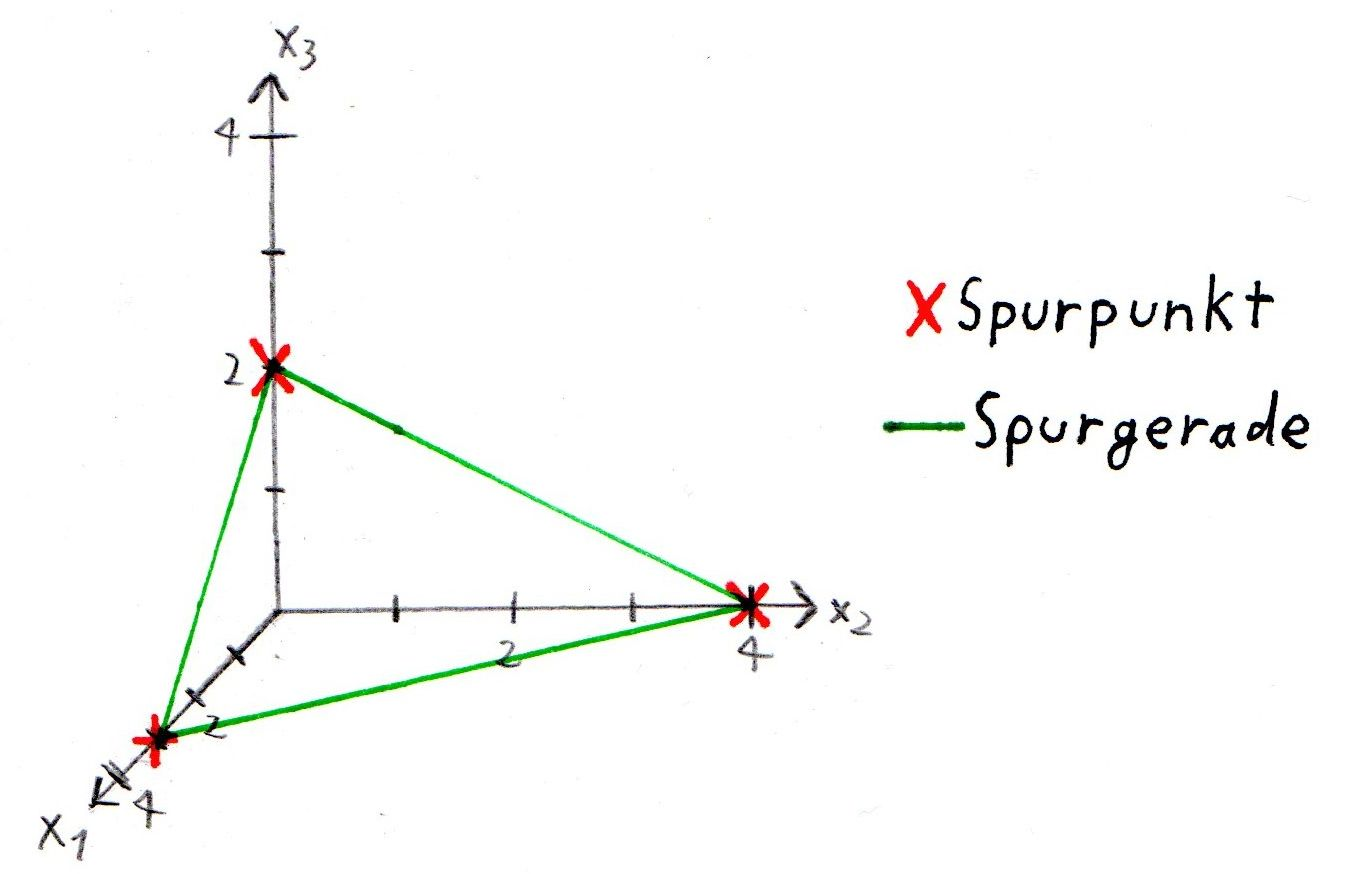
\includegraphics[scale=0.2]{Images/Spurpunkte.jpeg}
    		\caption{Spurpunkte und Geraden einer Ebene}
    	\end{figure}

		Um Ebenen darzustellen, nimmt man sich Spurpunkte bzw. -geraden zur Hilfe.
		Wenn nicht anders verlangt, raten wir zu den Spurpunkten. Das sind die Punkte,
		in denen die Ebene die Achsen schneidet. Man berechnet sie einfach, indem man
		(für das Schneiden mit der x-Achse) y=z=0 setzt und erhält so einen Wert für
		x. Mit den anderen Punkten, die man natürlich synchron dazu berechnet, spannt
		sich dann eine Ebene auf.\\
		Die Spurgeraden sind Geraden, die durch jeweils zwei Spurpunkte gehen. Diese
		benötigt man lediglich bei Ebenen, die in der Parameterform dargestellt sind.
		Dazu setzt man bei \(\vec{x}\) einfach eine Koordinate 0 und berechnet dann
		die Parameter in dieser Zeile.

	\subsection{einfache geometrische Formen im Raum}
		\todo[color=red]{Kasten für Formel hinzufügen}
		\todo[color=red]{Zusammenfassung-Kasten hinzufügen}
		\todo[color=red]{Signalwörter-Kasten hinzufügen}
		Jegliche Formen im Raum darzustellen, ist recht leicht. Hierzu setzt ihr
		einfach alle angegebenen Punkte ins Koordinatensystem ein und verbindet die
		Punkte (überlegt euch, welche Punkte überhaupt verbunden werden müssen, bei
		einem Quadrat ABCD ist es nicht sinnvoll, AC und BD zu verbinden).


	% Section Lagebeziehungen
	\section{Lagebeziehungen}
	\todo[color=purple]{Kasten für Formel hinzufügen}
	\todo[inline,color=red]{Zusammenfassung-Kasten hinzufügen}
	\todo[inline,color=red]{Signalwörter-Kasten hinzufügen}
	Zuletzt wollen wir noch die unterschiedlichen Lagebeziehungen besprechen.
	Manchmal wird explizit nach ihnen gefragt, manchmal brauchen wir sie aber auch,
	um im Wahlteil Anwendungsaufgaben beantworten zu können\footnote{wir werden
	hier nicht explizit auf die Erklärungen für Anwendungsaufgaben eingehen. Zum
	einen, weil es aus typografischen Gründen keinen Sinn macht und wir euch zum
	anderen nicht dadurch verwirren wollen. Im Kurs werden wir aber darauf
	eingehen.}. Die hier genannten Verfahren sind nicht die Einzigen, denn nicht
	nur ein Weg führt zur Lösung. Die hier besprochenen Wege sind unserer Meinung
	nach die Einfachsten. Wenn ihr mit eurer eigenen Methode aber besser zurecht
	kommt, ist es weniger sinnig, ausgerechnet unsere zu benutzen. Im Kurs werden
	wir bei Bedarf auch auf andere Wege eingehen.

	% Punkt - Punkt
	\subsection{Punkt - Punkt}
	\todo[color=purple]{Kasten für Formel hinzufügen}
	\todo[color=purple]{Zusammenfassung-Kasten hinzufügen}
	\todo[color=purple]{Signalwörter-Kasten hinzufügen}
	Diese Beziehung dürfte klar sein. Entweder haben wir den gleichen Punkt im Raum
	(was sofort erkennbar wäre) oder aber sie liegen örtlich auseinander. Dann kann
	man angeben, wie weit die Punkte entfernt sind, indem man einen Punkt vom
	anderen abzieht (Ziel minus Angriff) und von diesem neuen Vektor den Betrag
	berechnet, um zu berechnen, um den Abstand zu bestimmen.


	% Punkt - Gerade
	\subsection{Punkt - Gerade}
Hier wollen wir den kleinsten Abstand von der Geraden zum Punkt berechnen\footnote{tatsächlich gibt es ja unendlich viele Abstände, entscheidend ist aber in der Mathematik immer der Kürzeste.}.\\
Zunächst setzt ihr den Punkt in die Gerade ein, um zu überprüfen, ob dieser nicht sogar darauf liegt. Liegt er nicht dort, so müsst ihr zuerst eine Hilfsebene aufstellen. Der Richtungsvektor der Geraden entspricht dann dem Normalenvektor der Hilfsebene. Euer Punkt, der nicht auf der Geraden liegt, ist der Stützvektor der Ebene (somit stellt ihr sicher, dass ein rechter Winkel zwischen Gerade und der Strecke zum Punkt ist). Nun müsst ihr ermitteln, in welchem Punkt die Gerade die Hilfsebene durchstößt. Ab hier ist es lediglich eine \textbf{Punkt - Punkt} - Beziehung die ihr berechnen müsst.\\
Das ganze ist natürlich recht aufwändig und nimmt viel Zeit in Anspruch. Glücklicherweise gibt es aber eine einfachere Variante. Sie mag nicht so ersichtlich sein, auf den ersten Blick. Letztendlich müsst ihr aber lediglich die Formel auswendig lernen. Auf den Beweis und den Gedanken dahinter, werden wir im Kurs näher eingehen. Wir setzen dort dann den angegebenen Punkt \(\vec{x}\) ein, so wie den Stützvektor \(\vec{a}\) und den Richtungsvektor \(\vec{b}\) und bekommen den Abstand d (ist d=0, so liegt der Punkt natürlich auf der Geraden)\footnote{Vor allem durch das Kreuzprodukt scheint das ganze recht komplex auszusehen. Letztendlich ist aber auch das schnell eingeübt.}:
\[d=\frac{|(\vec{a}-\vec{x})\times \vec{b}|}{|\vec{b}|}\]


	% Punkt - Ebene
	\subsection{Punkt - Ebene}
	\todo[color=green]{Kasten für Formel hinzufügen}
	\todo[inline,color=red]{Zusammenfassung-Kasten hinzufügen}
	\todo[inline,color=red]{Signalwörter-Kasten hinzufügen}
	Den Abstand zwischen einem Punkt und einer Ebene berechnet man mit der
	Hesseschen Normalform / Koordinatenform. Ihr müsst für \(\vec{x}\) einfach den
	angegebenen Punkt (dessen Abstand ihr zur Ebene ermitteln wollt) einsetzen und
	habt sofort den Abstand. Zur Wiederholung:
	\formel{\[d=(\vec{a}-\vec{x})\cdot \hat{n} \mathrm{\ bzw\ }
	d=\frac{n_1x_1+n_2x_2+n_3x_3-w}{|\vec{n}|}\]}
	Ist der Abstand 0, so liegt der Punkt natürlich auf der Ebene.


	% Gerade - Gerade
	\subsection{Gerade - Gerade}
\todo[color=red]{Kasten für Formel hinzufügen}
\todo[color=red]{Zusammenfassung-Kasten hinzufügen}
\todo[color=red]{Signalwörter-Kasten hinzufügen}
Beim Betrachten der Lage zwischen zwei Geraden gibt es vier unterschiedliche Möglichkeiten, die wir prüfen müssen. Wir empfehlen euch, zuerst die Richtungsvektoren zu betrachten und dann zu prüfen, ob diese linear abhängig sind oder nicht.\\
\(\star\) Ist dies der Fall, so können sie entweder parallel sein oder liegen sogar aufeinander. Um das herauszufinden, ermittelt ihr einfach den Abstand von einer Geraden zu dem Stützpunkt der anderen Geraden (Beziehung \textbf{Punkt - Gerade}). Ist der Abstand 0, so sind die Geraden identisch, ansonsten sind sie parallel und haben den Abstand d.\\
\(\star\) Sind die Richtungsvektoren nicht linear abhängig, so sind sie windschief oder schneiden sich an einem Punkt. Hierzu setzt man zuerst beide Geraden gleich und löst das LGS. Geht es auf, so schneiden sie sich in diesem Punkt (setzt das s oder t bitte in die entsprechende Gerade ein, um zu schauen an welchen Punkt sie sich schneiden und gebt diesen an).\\
Schneiden sich die beiden Geraden nicht, so sind sie windschief. Dann ist wieder der kürzeste Abstand zwischen den Geraden anzugeben. Hier müsst ihr wieder eine Hilfsebene aufstellen. Diesmal sind die Richtungsvektoren der beiden Geraden die Spannvektoren der Hilfsebene (siehe \textbf{Parameterform}). Aus ihnen könnt ihr sofort die Normalen- oder Koordinatenform mit dem Normalenvektor angeben. Euer Punkt auf der Ebene ist dann einer der Stützvektoren. Der Abstand der Ebene zum Stützvektor (Beziehung \textbf{Punkt - Ebene}) der anderen Geraden ist dann der kleinste Abstand zwischen den windschiefen Geraden.


	% Gerade - Ebene
	\subsection{Gerade - Ebene}
	\todo[color=red]{Kasten für Formel hinzufügen}
	\todo[color=red]{Zusammenfassung-Kasten hinzufügen}
	\todo[color=red]{Signalwörter-Kasten hinzufügen}
	Bei dieser Beziehung gibt es 3 Möglichkeiten, die vorkommen können. Um
	herauszufinden, welche vorliegt, ist zu empfehlen, zunächst Richtungsvektor und
	Normalenvektor zu vergleichen. Man skalar multipliziert einfach diese beiden
	Vektoren und betrachtet das Ergebnis.\\

	\(\star\) Ist das Skalarprodukt 0, so sind die Vektoren orthogonal, sowie
	Gerade und Ebene parallel. Nun berechnet man den Abstand des Stützvektors der
	Gerade zur Ebene (Beziehung \textbf{Punkt - Ebene}). Ist der Abstand 0, so
	liegt die Gerade auf der Ebene, ansonsten kennen wir dessen Abstand d.\\

	\(\star\) Ist das Skalarprodukt nicht 0, so wird die Gerade die Ebene
	durchstoßen. Diesen Punkt kann man herausfinden, indem man in der
	Ebenengleichung \(\vec{x}\) durch die Geradengleichung ersetzt und das LGS
	löst.
	\emph{Vorsicht gilt bei der Winkelbestimmung!} Hier gilt nämlich im Gegensatz
	zu den anderen Lagebeziehungen folgende Formel ( \(\vec{n}\) ist der
	Normalenvektor, \(\vec{a}\) der Richtungsvektor):
	\[cos(\alpha)=\frac{|\vec{n}\cdot \vec{a}|}{|\vec{n}|\cdot |\vec{a}|}\]


	% Ebene - Ebene
	\subsection{Ebene - Ebene}
	\todo[color=red]{Kasten für Formel hinzufügen}
	\todo[color=red]{Zusammenfassung-Kasten hinzufügen}
	\todo[color=red]{Signalwörter-Kasten hinzufügen}
	Auch hier gibt es potentiell 3 Möglichkeiten. Zunächst vergleichen wir die
	Normalenvektoren und schauen, ob diese linear abhängig sind.\\

	\(\star\) Sind sie es, so sind die Ebenen natürlich parallel zueinander. Hier
	wird dann der Abstand von einem Stützvektor der Ebenen zur anderen Ebene
	berechnet (Beziehung \textbf{Punkt - Ebene}). Ist dieser Abstand 0, so sind die
	beiden Ebenen identisch. Ist der Abstand nicht 0, so haben wir 2 parallele
	Ebenen mit dem Abstand d zueinander.\\

	\(\star\) Sind die Normalen nicht linear abhängig, so haben wir die dritte
	Möglichkeit. Die Ebenen schneiden sich. Um die Schnittgerade zu ermitteln,
	setzt man die Ebenen gleich und erhält ein LGS, welches man (mit einer
	Variablen, welche unser 's' ist) löst.

	
	% Stochastik
	\chapter{Stochastik}
	In der Stochastik geht es darum, Wahrscheinlichkeiten zu berechnen und zu
	verstehen, was es mit ihnen auf sich hat. Es geht also um statistische
	Verteilungen, bei der man eine Wahrscheinlichkeit angeben kann, dass ein
	Ereignis eintritt. Die Idee dahinter ist nicht allzu schwer und die
	Aufgabenstellungen lassen sich meist auf euch bekannte Situationen, wie z.B.
	Würfel oder Ziehen aus einer Urne, herunterbrechen. Das größte Problem wird
	sein, festzustellen, welches Ereignis wir überhaupt betrachten müssen.

	% Section Begriffe
	\section{Begriffe}
	In der Stochastik tauchen einige neue Begriffe auf, die wir zunächst betrachten
	wollen, bevor wir diese dann anwenden.

	\subsection{Ereignis}
		\todo[color=red]{Kasten für Formel hinzufügen}
		\todo[color=red]{Zusammenfassung-Kasten hinzufügen}
		\todo[color=red]{Signalwörter-Kasten hinzufügen}
		Zunächst sollten wir klären, was ein Ereignis in der Stochastik ist.
		Betrachten wir, wie etwas ausgehen kann, so gibt es meistens mehrere
		Möglichkeiten, die eintreten können. Diese werden in diesem Zusammenhang auch
		Ereignisse genannt. Jedes mögliche Ereignis bekommt dann einen großen
		Buchstaben (manchmal mit Indizes) zugewiesen\footnote{Das liegt daran, dass
		man hier Mengen angibt und keine Zahlen oder Sonstiges. Falls ihr damit
		Probleme habt schaut euch nochmal das dazugehörige Kapitel im Vorgeplänkel
		an}. Grundsätzlich können in einem Ereignis mehrere Einzelereignisse stecken.
		Ist unser Ereignis, dass eine gerade Zahl gewürfelt wird, so schreibt man dies
		als
		\[A=\left\lbrace 2;\ 4;\ 6\right\rbrace \]
		Da unser Ereignis \(A\) eine Menge ist lässt sich das Gegenereignis, welches
		immer dann eintritt, falls \(A\) nicht eintritt, als \(\bar{A}\) angeben.

	\subsection{Ereignismenge}
		\todo[color=red]{Kasten für Formel hinzufügen}
		\todo[color=red]{Zusammenfassung-Kasten hinzufügen}
		\todo[color=red]{Signalwörter-Kasten hinzufügen}
		Die Ereignismenge ist die Menge aller Ereignisse\footnote{Also eine Menge
		aller möglichen Mengen.}. Nehmen wir an, dass wir Würfeln. Es gibt also sechs
		mögliche Ereignisse. So würde man die Ereignismenge wie folgt darstellen:
		\[\Omega=\left\lbrace A_1;\ A_2;\ A_3;\ A_4;\ A_5;\ A_6\right\rbrace \]
		Wird gefragt, wie viele Ereignisse möglich sind, gebt niemals
		\(\Omega=\ldots\) an, denn die Ereignismenge ist eine Menge und allein deshalb
		schon keine Zahl. Was ihr dann angebt müsst ist die Anzahl der Elemente, also
		die Kardinalität, der Ereignismenge:
		\[\#\Omega=6\]

	\subsection{Wahrscheinlichkeit}
		\todo[color=red]{Kasten für Formel hinzufügen}
		\todo[color=red]{Zusammenfassung-Kasten hinzufügen}
		\todo[color=red]{Signalwörter-Kasten hinzufügen}
		Unser Ziel wird zumeist sein, die Wahrscheinlichkeit eines Ereignisses
		anzugeben. Das Ergebnis kann dann als Bruch (meist am bequemsten), Dezimalzahl
		oder als Prozentzahl angeben werden. Die Wahrscheinlichkeit P, dass das
		Ereignis A eintritt, ist dann (als Beispiel):
		\[P(A)=\frac{1}{2}=0,5=50\%\]
		An dieser Stelle möchten wir noch auf zwei Sätze eingehen, die uns zum Teil
		viel Arbeit ersparen können. Zuerst sollten wir die Nichtnegativität
		betrachten. Das bedeutet einfach, dass wir voraussetzen, dass alle
		Wahrscheinlichkeiten positive Zahlen sind (was auch Sinn macht, keine
		negativen Wahrscheinlichkeiten zu haben). So gilt:
		\[P(A)\geq 0 \mathrm{,\ für\ alle\ A}\]
		Weiter ist logisch nachvollziehbar, dass eines aller möglichen Ereignisse
		eintreten muss. Deshalb gilt auch folgende Relation:
		\[P(\Omega)=P(A_1)+P(A_2)+ \ldots+ P(A_n)=1\]
		Aus der gleichen Logik entspringt auch der folgende Ausdruck, welcher uns viel
		Arbeit ersparen wird. Denn die Wahrscheinlichkeit, dass ein Ereignis eintrifft
		\emph{und} dass es nicht eintrifft sind \(100\%\)(=1) (also die
		Wahrscheinlichkeiten summiert). Oder umgeschrieben:
		\[P(A)=1-P(\bar{A})\]

	\subsection{Zufallsgröße X}
		\todo[color=red]{Kasten für Formel hinzufügen}
		\todo[color=red]{Zusammenfassung-Kasten hinzufügen}
		\todo[color=red]{Signalwörter-Kasten hinzufügen}
		Haben wir Situationen, in denen mehrfach 'gezogen' wird, so gibt unsere
		Zufallsgröße an, wie oft das gewählte Ereignis eintreten soll, z. B. welche
		k's in die Bernoulli-Formel eingesetzt werden. Dies können dann alle k's höher
		oder niedriger oder genau ein Wert sein. Darauf gehen wir später genauer ein.

	\subsection{mit / ohne Zurücklegen}
		\todo[color=red]{Kasten für Formel hinzufügen}
		\todo[color=red]{Zusammenfassung-Kasten hinzufügen}
		\todo[color=red]{Signalwörter-Kasten hinzufügen}
		Macht man mehr als eine Probe, so gibt es unterschiedliche Möglichkeiten, wie
		die Wahrscheinlichkeiten im nächsten Zug sind.\\
		
		\(\star\) Ein System, in dem die Wahrscheinlichkeiten immer gleich sind,
		nennen wir ein System mit Zurücklegen. Aus dem Urnenmodell ist das leicht
		nachvollziehbar. Ziehe ich eine bestimmte Farbe mit der Wahrscheinlichkeit
		P(A), lege die Kugel zurück, so haben wir die gleiche Situation wie zuvor und
		somit auch die gleiche Wahrscheinlichkeit. Am Beispiel des Würfels ist dies
		leicht klar zu machen\footnote{Das 'Zurücklegen' ist gerade in diesem
		Vergleich ein schlechter Begriff, da es nicht unbedingt mit Ziehen oder Legen
		zusammenhängen muss. Da man jedoch oft das Urnenmodell als Vergleich hat,
		behalten wir das trotzdem bei.}.\\
		
		\(\star\) Systeme ohne Zurücklegen haben genau diese Eigenschaft nicht. Nach
		jedem Ziehen liegt eine neue Situation vor. Deshalb muss für jeden neuen Zug
		die Wahrscheinlichkeit neu berechnet werden.

	\subsection{Geordnet / Ungeordnet}
		\todo[color=red]{Kasten für Formel hinzufügen}
		\todo[color=red]{Zusammenfassung-Kasten hinzufügen}
		\todo[color=red]{Signalwörter-Kasten hinzufügen}
		Ungeachtet der Wahrscheinlichkeiten in einem Zug ist entscheidend, ob unser
		System geordnet oder ungeordnet ist, um zu entscheiden, welche und wie viele
		Pfade zum Erfolg führen (worauf später genauer eingegangen wird). Ein
		geordnetes System ist zum Beispiel eine PIN-Nummer. Selbst wenn man die
		Ziffern kennt und dann in der falschen Reihenfolge eingetippt, kommt man nicht
		ans Ziel. In diesem Beispiel gibt es also nur einen Pfad für das Eintreten des
		Ereignisses.\\
		Dagegen ist das Lotto spielen ein ungeordnetes System. Entscheidend ist nicht,
		welche Kugel als erstes gezogen wird, sondern lediglich welche Zahlen.


	% Section Mathematische Grundlagen
	\section{Mathematische Grundlagen}
Hier werden noch kurz mathematische Grundlagen angesprochen, auf die wir nachher zurückgreifen. Abgesehen davon, solltet ihr euch vor allem noch einmal mit den Regeln des Bruchrechnens und den Potenzgesetzen vertraut machen.

\subsection{Fakultät}
Die Fakultät wird in der Mathematik als Abkürzung verwendet. Immer dann, wenn man viele aufeinanderfolgende natürliche Zahlen multipliziert, verwendet man sie. Definiert ist sie wie folgt:
\[n!=1\cdot 2\cdot \ldots \cdot (n-1)\cdot n\ \&\ 0!=1\]

\subsection{Binomialkoeffizient}
Später werden wir seinen Nutzen noch genauer sehen, jetzt brauchen wir erstmal nur dessen Definition
\[\binom{n}{k}=\frac{n!}{(n-k)!\cdot k!}\mathrm{\ für\ alle\ }k,n\in \mathbb{N}\]
Weiter gilt folgendes:
\[\binom{n}{0}=\binom{n}{n}=1,\ \binom{n}{k}=\binom{n}{n-k}\]
Für kleine $n$ könnt ihr den Binomialkoeffizienten schnell mit Hilfe eines Pascal'schen Dreiecks bestimmen.\\
$
\begin{array}{ccccccccccccccccccccc}
n=0 &  &  &  &  &  & 1 &  &  &  &  &  &  &  &  &  & \binom{0}{0} &  &  &  & \\ 
n=1 &  &  &  &  & 1 &  & 1 &  &  &  &  &  &  &  & \binom{1}{0} &  & \binom{1}{1} &  &  & \\ 
n=2 &  &  &  & 1 &  & 2 &  & 1 &  &  & \Leftrightarrow &  &  & \binom{2}{0} &  & \binom{2}{1} &  & \binom{2}{2} &  & \\ 
n=3 &  &  & 1 &  & 3 &  & 3 &  & 1 &  &  &  & \binom{3}{0} &  & \binom{3}{1} &  & \binom{3}{2} &  & \binom{3}{3} & \\ 
n=4 &  & 1 &  & 4 &  & 6 &  & 4 &  & 1 &  & \binom{4}{0} &  & \binom{4}{1} &  & \binom{4}{2} &  & \binom{4}{3} &  & \binom{4}{4}\\
 & && && && && && && && && && &\\
k= & &0& &1& &2& &3& &4& &0& &1& &2& &3& &4   
\end{array} 
$


	% Section Einmaliges Ziehen
	\section{Einmaliges Ziehen}
	\subsection{Bei gleicher Wahrscheinlichkeit}
		\todo[color=green]{Kasten für Formel hinzufügen}
		\todo[color=purple]{Zusammenfassung-Kasten hinzufügen}
		\todo[color=purple]{Signalwörter-Kasten hinzufügen}
		Die einfachste Variante wäre, dass wir lediglich einmal 'ziehen', bzw. eine
		einzige Stichprobe nehmen. Letztendlich lässt sich auch das mehrmalige
		Wiederholen als immer neue einzelne Stichprobe ansehen (wobei dann auch die
		Kombination zu beachten ist). Doch wie können wir die Wahrscheinlichkeit für
		einen einzelnen Versuch nun berechnen?\\
		Zuerst definiert man die unterschiedlichen Ereignisse, die eintreten können.
		Nun kommt die Anzahl der Ergebnisse in den Nenner und die Anzahl derer, die zu
		dem gesuchten Ereignis gehören, in den Zähler und schon hat man die
		Wahrscheinlichkeit:
		\formel{\[P(A)=\frac{Anzahl\ der\ Ereignisse\ von\ A}{Anzahl\ der\ gesamten\
		Ereignisse}=\frac{\#A}{\#\Omega}\]}
		Leichter verständlich wird das an einem	Beispiel. Haben wir zum Beispiel einen
		Würfel, ist unser Ereignis, dessen Wahrscheinlichkeit wir berechnen wollen,
		nehmen wir nun an: A: es wird eine gerade Zahl gewürfelt. Nun haben wir sechs
		mögliche Zahlen, welche gewürfelt werden können, wobei jedes gleich
		wahrscheinlich ist. Damit Ereignis A eintritt, muss eine 2, 4 oder 6 gewürfelt
		werden. Wir haben also drei 'Mini-Ereignisse' für A. Somit gilt
		\(P(A)=\frac{3}{6}=\frac{1}{2}=50\%\).
	
	\subsection{Bei unterschiedlichen Wahrscheinlichkeiten}
		\todo[color=green]{Kasten für Formel hinzufügen}
		\todo[color=purple]{Zusammenfassung-Kasten hinzufügen}
		\todo[color=purple]{Signalwörter-Kasten hinzufügen}
		Bei unterschiedlichen Wahrscheinlichkeiten für einzelne Ereignisse müssen
		diese in der Aufgabenstellung gegeben sein. Es ist somit uninteressant die
		Wahrscheinlichkeit für ein einzelnes Ereignis \(A_1\) zu berechnen. Meist ist
		dann die Frage mit welcher Wahrscheinlichkeit eine Kombination von Ereignissen
		eintritt. Dafür addiert man die Einzel-Wahrscheinlichkeiten zusammen:
		\formel{\[P(A)=P(A_1)+P(A_2)+\cdots+P(A_n)\]}
		Bei einer Kombination aus sehr vielen Ereignissen ist es oft leichter die
		Wahrscheinlichkeit mit Hilfe des Gegenereignisses zu bestimmen:
		\formel{\[P(A)=1-P(\bar{A})=1-(P(\bar{A}_1)+P(\bar{A}_2)+\cdots+P(\bar{A}_n))\]}


	% Section Mehrmaliges Ziehen
	\section{Mehrmaliges Ziehen}

\subsection{Pfade}
\todo[color=red]{Kasten für Formel hinzufügen}
\todo[color=red]{Zusammenfassung-Kasten hinzufügen}
\todo[color=red]{Signalwörter-Kasten hinzufügen}
Zieht man nun häufiger, so ist das Bestimmen der Wahrscheinlichkeit nicht auf den ersten Blick sichtbar. Um sich die Arbeit zu vereinfachen, zeichnet man ein Pfad-Diagramm. So beginnt man von einem Punkt und zeichnet dann davon so viele Linien, wie es mögliche Ereignisse gibt (an deren Ende kennzeichnet man, um welches es sich handelt; zur Übersichtlichkeit alle Ereignisse untereinander). Auf oder neben die Linien kommt dann die Wahrscheinlichkeit für die jeweiligen Ereignisse. Nun wird an jedem Ereignis das Gleiche wiederholt. Oft wird ein Pfad-Diagramm, wegen seines Aussehens, auch als 'Baum'-Diagramm und dessen Pfade als 'Äste' bezeichnet\\
Liegt ein System mit Zurücklegen vor, so bleibt die Wahrscheinlichkeit für die Ereignisse immer gleich (wie beim Würfeln). Ohne Zurücklegen wird das schwieriger. Haben wir 5 Kugeln, 2 weiße und 3 schwarze, so ist die Wahrscheinlichkeit eine Schwarze zu ziehen \(\frac{3}{5}\). Legen wir diese nicht zurück, so ist beim nächsten Schritt eine schwarze Kugel weniger, die man ziehen kann, also auch insgesamt eine weniger. Somit ist dann die Wahrscheinlichkeit \(\frac{2}{4}=\frac{1}{2}\).\\
Man muss im Übrigen nicht alle möglichen Pfade aufzeichnen. Beobachtet man, wie hoch die Wahrscheinlichkeit ist, dass man nur schwarze Kugeln zieht, so ist es nicht nötig, einen Pfad mit einer weißen Kugel weiter zu führen.

\subsection{Ereignisse bei mehrmaligem Ziehen}
\todo[color=red]{Kasten für Formel hinzufügen}
\todo[color=red]{Zusammenfassung-Kasten hinzufügen}
\todo[color=red]{Signalwörter-Kasten hinzufügen}
Beim mehrmaligen Ziehen besteht ein 'Mini-Ereignis' aus mehreren Ereignissen hintereinander, immer pro Zug einem. So ist ein Element (ein Gesamtereignis) aus mehreren Objekten zusammengesetzt. Also ist bei zweimaligem Münzwurf (1 für Kopf, 0 für Zahl) das Ereignis, dass einmal Kopf und einmal Zahl (ungeordnet) geworfen wird:
\[A=\lbrace (Zahl;Kopf),\ (Kopf;Zahl)\rbrace\]

\subsection{Pfadregeln}
\todo[color=red]{Kasten für Formel hinzufügen}
\todo[color=red]{Zusammenfassung-Kasten hinzufügen}
\todo[color=red]{Signalwörter-Kasten hinzufügen}
\(\star\) Nun haben wir mehrere Pfade, die uns zur Verfügung stehen. Zunächst legen wir ein Augenmerk darauf, wie hoch die Wahrscheinlichkeit für \underline{einen} gesamten Pfad ist. Nehmen wir an, wir ziehen 2 mal und die Wahrscheinlichkeit für beide Ereignisse, die pro Ziehen stattfinden können, beträgt \(\frac{1}{2}\). Für die Wahrscheinlichkeit eines Pfades (zum Beispiel man würfelt 2-mal hintereinander eine gerade Zahl) gilt dann:
\[P(A)=P(A_1) \cdot P(A_2) \cdot \ldots\]
\(A_1\) ist das erste Mal 'iehen', \(A_2\) das zweite Mal, usw.. In unserem Beispiel wäre dann die Wahrscheinlichkeit für einen Pfad mit dem Ereignis A: \(P(A)=\frac{1}{2} \cdot \frac{1}{2}=\frac{1}{4}=25\%\). Da alle Pfade gleich wahrscheinlich sind, wir 4 Pfade haben und eines der Ereignisse immer eintreten muss, ist das Ergebnis auch schlüssig.\\
\(\star\) Nun kann es vorkommen (vor allem bei ungeordneten Systemen!), dass mehrere Pfade zum Erfolg führen. Wollen wir zum Beispiel wissen, wie hoch die Wahrscheinlichkeit ist, dass wir nur gerade oder nur ungerade Zahlen Würfeln, so liegen zwei mögliche Ereignisse vor. Die Wahrscheinlichkeit, dass das Ereignis (der Pfad) A oder B vorliegt, ist dann:
\[P(A\cup B)=P(A)+P(B)\]
In unserem Fall also \(P(C)=\frac{1}{4}+\frac{1}{4}=\frac{1}{2}=50\%\). Da alle Pfade gleichwertig sind und 2 von 4 auf das Ereignis zutreffen, ist auch das ersichtlich.

\subsection{Reduktion von möglichen Ereignissen}
\todo[color=red]{Kasten für Formel hinzufügen}
\todo[color=red]{Zusammenfassung-Kasten hinzufügen}
\todo[color=red]{Signalwörter-Kasten hinzufügen}
Um sich Arbeit zu sparen, lohnt es sich, Ereignisse zusammenzufassen. So will man in den meisten Fällen wissen, ob ein Ergebnis eintritt oder nicht. 
Nehmen wir wieder das Beispiel mit dem Würfel. So wäre das Eintreten des Ereignisses A hier, dass wir eine gerade Zahl würfeln. Das Gegenereignis \(\overline{A}\) ist dann das Würfeln einer ungeraden Zahl (wäre aber - auch umgekehrt - genau so richtig). Anstatt hier also sechs einzelne Ereignisse zu haben, können wir das auf zwei Ereignisse reduzieren (jeweils pro Ziehen).\\
Das ganze nennt sich auch \textbf{Bernoulli-Versuch}, welcher in den meisten der Aufgaben realisierbar ist.


	% Section häufiges Ziehen
	\section{häufiges Ziehen}
	In den meisten Fällen wird in den Aufgabenstellungen relativ häufig 'gezogen'.
	So häufig, dass das 'Pfade aufzeichnen' viel zu unübersichtlich wird. Jedoch
	gibt es hier einige Tricks, die wir hier noch einmal zusammenfassen wollen, für
	die vier möglichen Situationen, die es in der diskreten Statistik gibt.

	\subsection{mit Zurücklegen - geordnet}
		\todo[color=red]{Kasten für Formel hinzufügen}
		\todo[color=red]{Zusammenfassung-Kasten hinzufügen}
		\todo[color=red]{Signalwörter-Kasten hinzufügen}
		Hier lassen sich Wahrscheinlichkeiten mit etwas Überlegung einfach bestimmen,
		da die Wahrscheinlichkeit pro Versuch sich nicht verändert. Dank des
		Kommutativgesetzes (= des Vertauschungsgesetzes) kann man die
		Wahrscheinlichkeiten P einzeln multiplizieren (also hoch k nehmen) und
		multipliziert das dann mit den Gegenwahrscheinlichkeiten (hoch dem Rest n-k,
		also so oft das Ergebnis nicht eintritt). Soll bei n Versuchen k mal der
		Erfolg eintreten (deshalb P(X=k)), gilt in dem Fall
		\[P(E)=P(A)^k\cdot P(\overline{A})^{n-k} \Rightarrow\] \[P(X=k)=p^k\cdot
		(1-p)^{n-k}\]
		da ja die Wahrscheinlichkeit für das Nicht-Eintreten pro Pfad mitberechnet
		werden muss. Ob alle Ereignisse nun immer zuerst und danach alle
		Gegenereignisse eintreten oder ob das ganze gemischt auftritt, ist für die
		Berechnung aufgrund des Kommutativgesetzes, irrelevant. Die Wahrscheinlichkeit
		bleibt gleich, da wir durch das rein mathematische Umordnen den Pfad nicht
		verändern oder verlassen.

	\subsection{mit Zurücklegen - ungeordnet (Bernoulli-Formel)}
		\todo[color=red]{Kasten für Formel hinzufügen}
		\todo[color=red]{Zusammenfassung-Kasten hinzufügen}
		\todo[color=red]{Signalwörter-Kasten hinzufügen}
		\(\star\) Damit ein Bernoulli-Versuch vorliegt, muss folgendes gelten: Man
		kann den Versuch auf Eintreten \& Nicht-Eintreten reduzieren, da die
		Wahrscheinlichkeiten immer gleich bleiben (mit Zurücklegen) und die
		Reihenfolge irrelevant ist (ungeordnet).\\
		
		\(\star\) Haben wir einen Bernoulli-Versuch, so ist die Wahrscheinlichkeit für
		einen Pfad ebenso zu berechnen, wie im geordneten Fall. Jedoch gibt es mehrere
		Pfade, welche für ein Ereignis E geltend sind. Die Reihenfolge ist wieder
		unbedeutend, wie beim Lottospielen. Man addiert diese dann. Da alle Ereignisse
		die gleiche Wahrscheinlichkeit haben, kann man die Anzahl der dazugehörigen
		Pfade auch multiplizieren. Doch wie viele sind das? Nun, hier ist wieder der
		Binomialkoeffizient gefragt. Somit ergibt sich bei n Versuchen mit k Treffern
		\[P(X=k)=B(k,p,n)=\binom{n}{k}\cdot p^k\cdot (1-p)^{n-k}\] wobei 1-p die
		Gegenwahrscheinlichkeit vom Ereignis ist.


	% Section mindestens / höchstens
	\section{mindestens / höchstens}
	\todo[color=green]{Kasten für Formel hinzufügen}
	\todo[inline,color=red]{Zusammenfassung-Kasten hinzufügen}
	\todo[inline,color=red]{Signalwörter-Kasten hinzufügen}
	In einigen Aufgaben wird danach gefragt, wie hoch die Wahrscheinlichkeit ist,
	dass bei n mal ziehen mindestens / höchstens k mal das Ereignis eintrifft.
	Sollen Beispielsweise höchstens 5 Bauteile von 50 defekt sein, so müssen wir
	alle Pfade, in denen 1, 2, 3, 4 und 5 Bauteile defekt sind, berechnen und
	addieren. Bei mindestens folgt das selbe analog, nur eben dass alle mit 5 oder
	höher, addiert werden. So berechnet sich das Ganze wie folgt:
	\formel{\[\mathrm{\underline{Höchstens}: }P(X\leq k)=P(X=0)+P(X=1)+\ldots
	+P(X=k)\]
	\[\mathrm{\underline{Mindestens}: }P(X\geq k)=P(X=k)+P(X=k+1)+\ldots+P(X=n)\]}
	Ist die Wahrscheinlichkeit für 'weniger als' oder 'mehr als' gefragt, so
	schreibt man dies als \(P(X<k)\mathrm{\ bzw.\ }P(X>k)\)\footnote{Beachtet bei
	der Taschenrechner Eingabe, dass dort immer $P(X\leq k)$ oder $P(X\geq k)$
	gefragt ist!}.\\
	Ihr könnt euch auch oft viel Arbeit ersparen, wenn ihr auch hier die Formel
	\(P(A)=1-P(\overline{A})\) beachtet. Denn sollte in unserem vorherigen Beispiel
	die Wahrscheinlichkeit berechnet werden, dass mindestens 45 Bauteile
	funktionieren sollen, so ist dies das gleiche, wie wenn man die
	Wahrscheinlichkeit für höchstens 4 Bauteile berechnet und diese von 100\%
	abzieht (denn das ist die Gegenwahrscheinlichkeit dazu).


	% Section einseitiger Signifikanztest
	\section{einseitiger Signifikanztest}
	\todo[color=purple]{Kasten für Formel hinzufügen}
	\todo[color=purple]{Zusammenfassung-Kasten hinzufügen}
	\todo[color=purple]{Signalwörter-Kasten hinzufügen}
	Signifikanztests dienen der Überprüfung einer Behauptung, der Nullhypothese,
	und fallen in die Gruppe der „statisitschen Tests“.\\
	Stellt man die eine sog. Nullhypothese auf, so behauptet man, der Sachverhalt
	sei mit einer exakten Wahrscheinlichkeit verteilt, dies ist wie vorgehend
	erwähnt, lediglich eine Behauptung und spiegelt nicht die Realität wieder.\\
	Da bei einer Überprüfung lediglich eine Stichprobe entnommen wird und nicht die
	Gesamtheit aller Ereignisse betrachtet werden kann, ist es nicht möglich, die
	Behauptung vollständig zu be- oder widerlegen.\\
	Es ist lediglich möglich, die Wahrscheinlichkeit einer bestimmten Lösungsmenge
	für das Scheitern von \(H_1\) zu berechnen.\\
	Als Beispiel dient uns eine Lieferung an Elektronikartikeln. Der Hersteller
	gibt an, dass höchstens 10\% der 500 Teile defekt sind. Man betrachtet hier den
	Grenzfall. Das Ergebnis ist binomial verteilt.\\
	Für das Abitur in Baden-Württemberg sind nur die einseitigen Signifikanztests
	relevant.
	Hierbei schaut man sich an, wie sehr man sich irrt, wenn man annimmt, dass mit
	einer bestimmten Wahrscheinlichkeit höchstens, bzw. mindestens, eine bestimmte
	Anzahl an Nicht-Treffern auftritt. Ist diese entsprechend klein, kann man dann
	getrost von der eigentlichen Hypothese ausgehen.

	% Begriffe
	\subsection{Begriffe}
Zunächst sollten wir uns noch einmal die Begriffe klar machen, um zu wissen, worüber wir nachher reden.\\
\(\star\) Die angenommene (Einzel)Wahrscheinlichkeit \(p_0\) wird nachher - wie gewohnt - in die Bernoulliformel eingesetzt.\\
\(\star\) \(P(X\leq k) \mathrm{\ bzw.\ } P(X\geq k)\) sind unsere berechneten (Gesamt)Wahrscheinlichkeiten (das ist die Wahrscheinlichkeit, dass diese (Gegen)Hypothese stimmt).\\
\(\star\) k ist unser Grenzwert bei der Stichprobe, ab dem unsere aufgestellte Bedingung gilt, bzw. auf der anderen Seite, nicht mehr gilt.\\
\(\star\) \(H_0\) werden wir Nullhypothese nennen. Das ist die, welche wir annehmen.\\
\(\star\) \(H_1\) ist entsprechend die Gegenhypothese, die eintritt, falls wir falsch liegen (sie ist also das Gegenteil von \(H_0\)).\\
\(\star\) \(\alpha\) ist unsere Irrtumswahrscheinlichkeit. Diese wird meistens vorher festgelegt und gilt als Grenze. Liegt die berechnete Wahrscheinlichkeit darüber muss $H_0$ verworfen werden.\\
\(\star\) n ist die Anzahl an Stichproben, welche wir beim Versuch nehmen. k ist dann die Anzahl von Stichproben, bei denen das Ereignis eingetroffen ist (wie das bei den Wahrscheinlichkeiten selbst schon bekannt ist).


	% Die Idee
	\subsection{Die Idee}
	\todo[color=red]{Kasten für Formel hinzufügen}
	\todo[color=red]{Zusammenfassung-Kasten hinzufügen}
	\todo[color=red]{Signalwörter-Kasten hinzufügen}
	Die Idee dahinter ist auf den ersten Blick etwas abstrakt. Für das Abitur muss
	man sie nicht unbedingt verstanden haben, wir werden aber trotzdem versuchen,
	sie klar zu machen. Man versucht zu ermitteln, wie wahrscheinlich die
	Gegenhypothese ist, also wie sehr es sein kann, dass wir richtig liegen, wenn
	wir die Gegenhypothese \(H_1\) annehmen. Ist diese gering, so ist die
	Nullhypothese \(H_0\) entsprechend wahrscheinlich. Genau betrachten wir
	übrigens, wie wahrscheinlich \(p_0\) ist.\\
	Die Rechnung an sich verhält sich analog zu Bernoulli Versuchen mit höchstens
	oder mindestens mit der Ausnahme, dass beim Signifikantest die Grenze \(k\)
	gesucht und nicht gegeben ist. Das schwerste an den Signifikantests ist die
	Entscheidung, ob es sich um einen links- oder rechtsseitigen Test handelt.


	% Rechnung
	\subsection{Rechnung}
\subsubsection{Die Hypothesen \& links- oder rechtsseitiger Test}
Als erstes müssen wir aus dem Aufgabentext herauslesen, wie unsere Nullhypothese $H_0$ aussieht, falls sie nicht gegeben ist.\\
In unserem Beispiel lautet $H_0:\ p_0\leq 0.10$. Um nun unsere alternative Hypothese aufzustellen müssen wir von einer schlechteren Wahrscheinlichkeit ausgehen. Es gilt also: $H_1:\ p>0.10$.\\
Der nächste Schritt ist die Entscheidung, ob es sich um eine links- oder rechtsseitigen Test handelt. Dabei gibt es eine klare Regel\footnote{Verschiebt sich der Graph der Verteilung nach links ist es ein linksseitiger Test, verschiebt er sich nach rechts ist es ein rechtsseitiger Test}\\
$\star$ Gilt $p>p_0$ handelt es sich um einen rechtsseitigen Test.\\
$\star$ Gilt $p<p_0$ handelt es sich um einen linksseitigen Test.\\
\subsubsection{Die Gleichungen}
Bei einem linksseitigem Test werden alle Wahrscheinlichkeiten bis zu unserem Grenzwert $k$ addiert und hier kommt das einzig mathematisch Neue die Ungleichung:
\[P(X\geq k)=B(n,p_0,0)+B(n,p_0,1)+\ldots+B(n,p_0,k) \leq \alpha\]
Bei einem Rechtsseitigen Test entsprechen umgekehrt:
\[P(X\leq k)=B(n,p_0,k)+B(n,p_0,k+1)+\ldots+B(n,p_0,n) \leq \alpha\]
Nun muss die passende Gleichung nur noch nach $k$ aufgelöst werden. Dabei gibt es zwei Möglichkeiten\footnote{Für Maple Schüler bietet sich der Summen-Weg an, da dieser von Maple übersichtlicher dargestellt wird. GTR Schüler müssen den Weg über die Wertetabelle nehmen. CAS Schüler haben die Auswahl, wir empfehlen allerdings den Weg über die Wertetabelle, da es sein kann, dass der CAS bei der Summe zu lange rechnet.}:\\
$\star$ Das Umschreiben der Gleichung als Summe:
\[\text{Für den linksseitigen Test:}\sum_{i=0}^{k}B(n,p_0,i)\leq \alpha,\ \text{Für den rechtsseitigen Test:}\sum_{i=k}^{n}B(n,p_0,i)\leq \alpha\]
$\star$ Oder das Lösen mit Hilfe einer Wertetabelle.
Bei unserem Beispiel handelt es sich um einen rechtsseitigen Test da kein $\alpha$ in der Aufgabestellung gegeben war. Wir haben mit $\alpha=0.05$\footnote{Standardwerte für $\alpha$ sind $0.01,\ 0.05$ und $0.10$} gerechnet. Die Berechnungen ergeben:
\[P(X\geq 61)=0.0612,\ P(X\geq 62)=0.0465\] 


	% Auswertung des Ergebnisses
	\subsection{Auswertung des Ergebnisses}
Im Abitur wird meistens \(\alpha\) angegeben. Bei den einseitigen Signifikanztests können wir also genau betrachten, wann die Wahrscheinlichkeit für die Gegenhypothese diesen Wert überschreitet oder unterschreitet. Daher gibt die Ungleichung direkt an, welcher Ablehnungsbereich $\bar{A}$ und welcher Annahmebereich $A$ für unsere Nullhypothese $H_0$ gilt. Je nach dem, wie wichtig es ist, ob man \(\alpha\) vertraut, würde man selbiges verändern. Ein großer Wert für $\alpha$ bedeutet, dass wir uns mit einer größeren Wahrscheinlichkeit irren, was aber dazu führt, dass unser Annahmebereich größer ist. Aufgrund dessen können wir also eine eindeutige Antwort darauf finden, ob die Behauptung zutrifft oder nicht.\\
Bei unserem Beispiel schließen wir daraus, dass $H_1$ für mindestens 62 kaputte Teile zutrifft, also $H_0$ verworfen werden muss.
Es ergeben sich für $H_0$ ein Annahmebereich $A=\{0,\cdots,\ 61\}$, sowie ein Ablehnungsbereich $\bar{A}=\{62,\cdots,\ 500\}$
 
	
	\todo[inline,color=red]{"Anhang Taschenrechner" einfügen}
\end{document}